\documentclass[11pt]{article}

% Language setting
% Replace `english' with e.g. `spanish' to change the document language
\usepackage[english]{babel}

% Set page size and margins
% Replace `letterpaper' with `a4paper' for UK/EU standard size
\usepackage[a4paper,top=3cm,bottom=4cm,left=3cm,right=3cm,marginparwidth=1.75cm]{geometry}

% Useful packages
\usepackage{amsmath}
\usepackage{graphicx}
\usepackage{setspace}
\usepackage{amssymb}
\usepackage[font=small,labelfont=bf]{caption}

\usepackage[colorlinks=true, allcolors=blue]{hyperref}

\title{Deep Learning Approaches to Reduced Order Modeling of Parametrized Partial Differential Equations\\ \vspace{0.5em} \textit{\normalsize Report for the PhD course Mathematical Methods for Deep Learning\\ \vspace{-0.7em}  by Marco Verani and Edie Miglio}}
\author{Matteo Caldana}

\begin{document}
\maketitle

\begin{abstract}
Deep learning (DL) has been recently applied to reduced order models (ROM) as a way to surpass the severe limitations when dealing with nonlinear time-dependent parameterized PDEs. Indeed, conventional ROMs, such as proper orthogonal decomposition, are strongly anchored to the assumption of modal linear superimposition they are based on. The advantage of using a DL-based technique is that the learning is done in a non-intrusive way. Two models are gaining traction: DL-ROM and USM-Net. The former has shown great results in terms of accuracy but heavily relies on a series of snapshots solution of a full order model. The latter, instead, can learn both in black-box and in gray-box mode and does not rely upon a discretization at a fixed number of points. I will review the theory behind DL-ROM and USM-Nets and I will present a novel application in shape varying domains  parameterized by a NURBS surface. Code is available at \href{https://github.com/MatteoCaldana/mm4dl-project}{mm4dl-project}.
\end{abstract}


\section*{Introduction}
Traditional high-fidelity techniques, such as the Galerkin-finite element method, are too expensive for performing the numerical approximation of parametrized PDEs in real time. The main goal of reduced order modeling (ROM) techniques is to replace the full order model (FOM) with a model featuring a much lower dimension, yet capable to express the physical features of the problem at hand. In this context, the reduced basis (RB) method represents one of the most popular options \cite{quarteroni2015reduced}. The basic assumption underlying the RB method is that the solution of a parametrized PDE lies on a low-dimensional manifold, which can be approximated by a linear trial subspace spanned by a set of basis functions \cite{benner2017model}, built from a set of FOM snapshots employing, e.g., proper orthogonal decomposition (POD). In this case, the ROM approximation is given by the linear superimposition of POD modes, whose degrees of freedom result from the solution of a low-dimensional, non-linear, dynamical system. Unfortunately, when the physical
behavior is strongly affected by parametric dependence, linear ROMs might experience computational bottlenecks due to propagation in time of coherent structures. Namely, this happens in
transport and wave-type phenomena, and convection-dominated flows. This issues might also affect the ROM stability \cite{ballarin2015supremizer}.\\


Neural networks based ROMs (DL-ROMs) were recently proposed in \cite{fresca2021comprehensive} as a strategy for constructing ROMs for nonlinear time-dependent parametrized PDEs in a non-intrusive way. The trial manifold is learnt by means of the decoder function of a convolutional autoencoder (CAE) neural network, whereas the reduced dynamics through a deep feedforward neural network, and the encoder function of the CAE. It has been shown that DL-ROMs outperform the RB method in terms of numerical accuracy and computational efficiency during the online stage.\\

Another novel surrogate model that was recently introduced is USM-Nets \cite{regazzoni2022}. They are based on dense feed forward neural networks (DFNNs) and
can learn the solution manifold of a given parameterized PDE. Notably, these surrogate models do not necessarily rely on a FOM for surrogating the solution map.\\

This report is structured as follows. In Section~\ref{sec:review} I review the theory behind DL-ROM and then I briefly touch on USM-Nets.  In Section~\ref{sec:numericres} I will showcase two completely novel applications in domains of parameterized shape. Namely, I will present a test case of a Laplacian solved in a deformed quarter of a ring and the Scordelis-Lo Roof benchmark for elasticity on a shell \cite{reddy2006theory}. In both cases the domain is parameterized by a NURBS surface \cite{piegl1996nurbs}. Finally, in Section~\ref{sec:discussion} I discuss the results and draw some conclusions.

\section{Review of Literature}\label{sec:review}
Let me introduce the common settings for DL-ROM and USM-Net. Consider a space dependent physical quantity
$$\mathbf u: \mathbf x\in\Omega_{\boldsymbol \mu_g}\subset\mathbb R^d, d=2,3 \mapsto \mathbf u( \mathbf x) \in \mathbb R^k, k=1,2,... \; .$$
$\mathbf u( \mathbf x)$ depends on a set of physical parameter $\boldsymbol \mu_p\in\mathcal P_p \subset \mathbb R^{n_p}$ 
and a set of shape parameters $\boldsymbol \mu_g\in\mathcal P_g \subset\mathbb R^{n_g}$ 
that explicitly defines a varying domain $\Omega_{\boldsymbol \mu_g}$. 
For short
$$\boldsymbol \mu = (\boldsymbol \mu_p, \boldsymbol \mu_g) \in \mathcal P = \mathcal P_p \times \mathcal P_g \subset \mathbb R^{N_\mu = n_p + n_g}.$$ 
I write $\mathbf u( \mathbf x; \boldsymbol \mu)$ to stress the dependency on parameters $\boldsymbol \mu$.

Suppose there is a physical process that determines $\mathbf u(\mathbf x; \boldsymbol \mu)$ and can be described as a differential boundary value problem. If the problem is well posed, given $\boldsymbol  \mu$ there exists a unique solution 
$$\mathbf u(\cdot; \boldsymbol \mu): \Omega_{\boldsymbol \mu} \rightarrow \mathbb R^k, \quad \forall \boldsymbol \mu \in \mathcal P.$$
This solution can be numerically approximated by 
$$\mathbf u_h(\boldsymbol \mu) = \mathbf u(\mathbf x^i; \boldsymbol \mu) \in \mathbb R^{N_h \times k}, \, \{\mathbf x^i\}_{i=1}^{N_h} \subset \mathbb R^d, \quad \forall \boldsymbol \mu \in \mathcal P$$
through a FOM ($\{\mathbf x^i\}_{i=1}^{N_h}$ are fixed), for instance with finite elements, finite volumes or spectral elements.

Then, DL-ROM and USM-Nets try to achieve to slightly different objectives. In the former the goal is the efficient numerical approximation of the map of solutions (also known as solution manifold, see Figure~\ref{fig:manifold})
$$\boldsymbol \mu \mapsto \mathbf u_h(\boldsymbol \mu) \in \mathbb R^{N_h \times k} \quad \forall \boldsymbol \mu \in \mathcal{P}.$$
USM-Nets, instead, surrogate the map 
$$(\mathbf x, \boldsymbol \mu) \mapsto \mathbf u(\mathbf x; \boldsymbol \mu) \in \mathbb R^{k}  \quad \forall \boldsymbol \mu \in \mathcal{P}, \mathbf x \in \Omega_{\boldsymbol \mu}$$
so that it is possible to employ solutions from different FOM or use physical measurements or even learning in a non-supervised manner.
\begin{figure}
\centering
\begin{minipage}{.47\textwidth}
  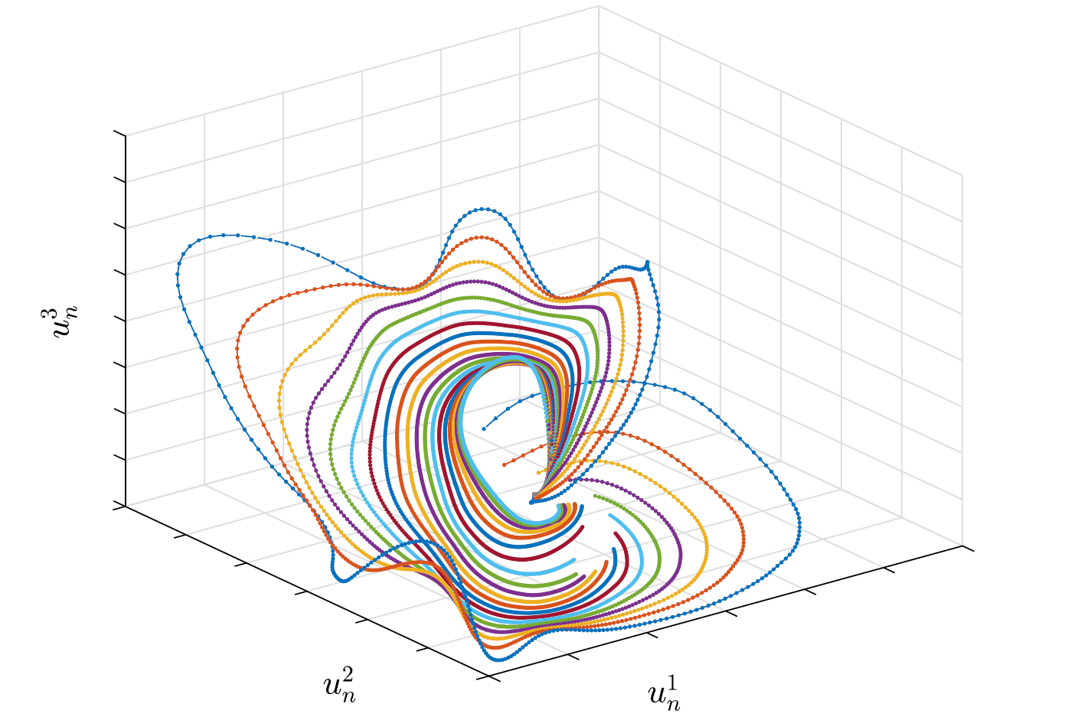
\includegraphics[width=1.\linewidth]{imgs/manifold.png}
  \caption{A two-dimensional manifold embedded in $\mathbb R^3$. Each curve represents the time-evolution of the first
three components of the solution of a (nonlinear) parametrized PDE for a fixed parameter value $\mu$.}
    \label{fig:manifold}
\end{minipage}%
\hfill
\begin{minipage}{.47\textwidth}
  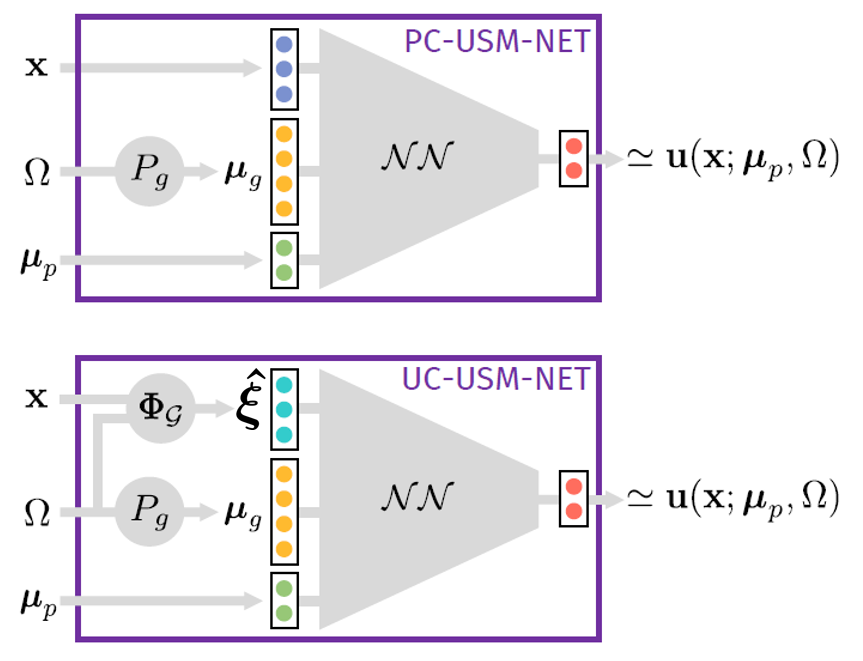
\includegraphics[width=1.0\textwidth]{imgs/usm-net-original.png}
    \caption{Architecture of a PC-USM-Net (top) and of a UC-USM-Net
(bottom).}
    \label{fig:usm-net}
\end{minipage}
\end{figure}

\subsection{DL-ROM}\label{sec:dlrom}
Differently from what done in the original paper \cite{fresca2021comprehensive}, I am formally treating time $t$ like any other parameter $\boldsymbol \mu$. Indeed, for the DL-ROM model, time does not have any preferential treatment with respect to other parameters: you can think of appending $t$ to the vector of parameters $\boldsymbol \mu$.
\subsubsection{Dimensionality Reduction}
For sake of simplicity, in the following I will consider $k=1$. Given the dimension of the intrinsic coordinates $n$ s.t. $N_\mu \ll n \ll N_h$, the most common way of building a ROM relies on two ingredients:
\begin{itemize}
    \item A nonlinear, differentiable function $\Psi_h: \mathbb R^{n} \rightarrow \mathbb R^{N_h}$ that maps a vector in a low dimensionality space of intrinsic coordinates to the full order solution. 
    \item A nonlinear map $\varphi_n : \mathbb R^{N_\mu} \ \rightarrow \mathbb R^{n}$ that maps the parameters to the intrinsic coordinates.
\end{itemize}
\paragraph{Linear Dimensionality Reduction for Time-Dependent Problems.} Just for this paragraph I assume the aim is to solve
\begin{equation}
\label{eq:ode}
    \begin{cases}
    \dot{\mathbf u_h}(t, \boldsymbol \mu) = \mathbf g(t, \mathbf u_h(t, \boldsymbol \mu); \boldsymbol \mu), \quad t\in(0,T)\\
    \mathbf u_h(0, \boldsymbol \mu) = \mathbf u_0(\boldsymbol \mu)
    \end{cases}
\end{equation}
Then, the most common way to build ROM is the following choice of $\Psi_h$: 
$$\Psi_h : \mathbf u_n \mapsto \tilde{\mathbf u}_h = V \mathbf u_n, V \in \mathbb R^{N_h \times n},$$
where $V$ is computed as follows. Consider $N_s$ instances of $(t, \boldsymbol \mu) \in \mathbb R \times \mathcal P$, define $S\in \mathbb R^{N_h\times N_s}$
$$S=[\mathbf u_h(t; \boldsymbol \mu^1)|...|\mathbf u_h(t; \boldsymbol \mu^{N_s})],$$
and define the positive definite matrix $X_h \in \mathbb R^{N_h\times N_h}$ encoding a suitable norm (e.g. the energy norm), admitting the Cholesky factorization $X_h=H^TH$. Moreover, compute the SVD factorization of $HS$
$$HS=U\Sigma Z^T,$$
where $U=[\boldsymbol \zeta_1|...|\boldsymbol \zeta_{N_h}] \in \mathbb R^{N_h\times N_h}$, and $\Sigma$ has on the diagonal the singular values ordered in decreasing order. Then
$$V=[H^{-1}\boldsymbol \zeta_1|...|H^{-1}\boldsymbol \zeta_{N_h} ].$$
It can be proven that $V$ provides the best reconstruction of the snapshots among all possible $n$-dimensional linear subspaces. In this case the map $\varphi_n$ is defined by the solution a system of ODEs of dimension $n$. Namely, by imposing that the residual
\begin{equation}
    \mathbf r_h(V \mathbf u_n(t, \boldsymbol \mu)) = V \dot{\mathbf u_n}(t, \boldsymbol \mu) - \mathbf g(t, V \mathbf u_n(t, \boldsymbol \mu); \boldsymbol \mu)
\end{equation}
to Eq.\ref{eq:ode}, the following ROM is obtained
\begin{equation}
        \begin{cases}
    Y^\top V \dot{\mathbf u_n}(t, \boldsymbol \mu) = Y^\top \mathbf g(t, \mathbf u_n(t, \boldsymbol \mu); \boldsymbol \mu), \quad t\in(0,T),\\
    \mathbf u_n(0, \boldsymbol \mu) = (Y^\top V)^{-1} Y^\top \mathbf u_0(\boldsymbol \mu).
    \end{cases}
\end{equation}
If $Y = V$, a Galerkin projection is performed, while the case $Y \neq V$ yields a more general Petrov-Galerkin projection.
\subsubsection{The DL-ROM Model}
\begin{figure}[t]
    \centering
    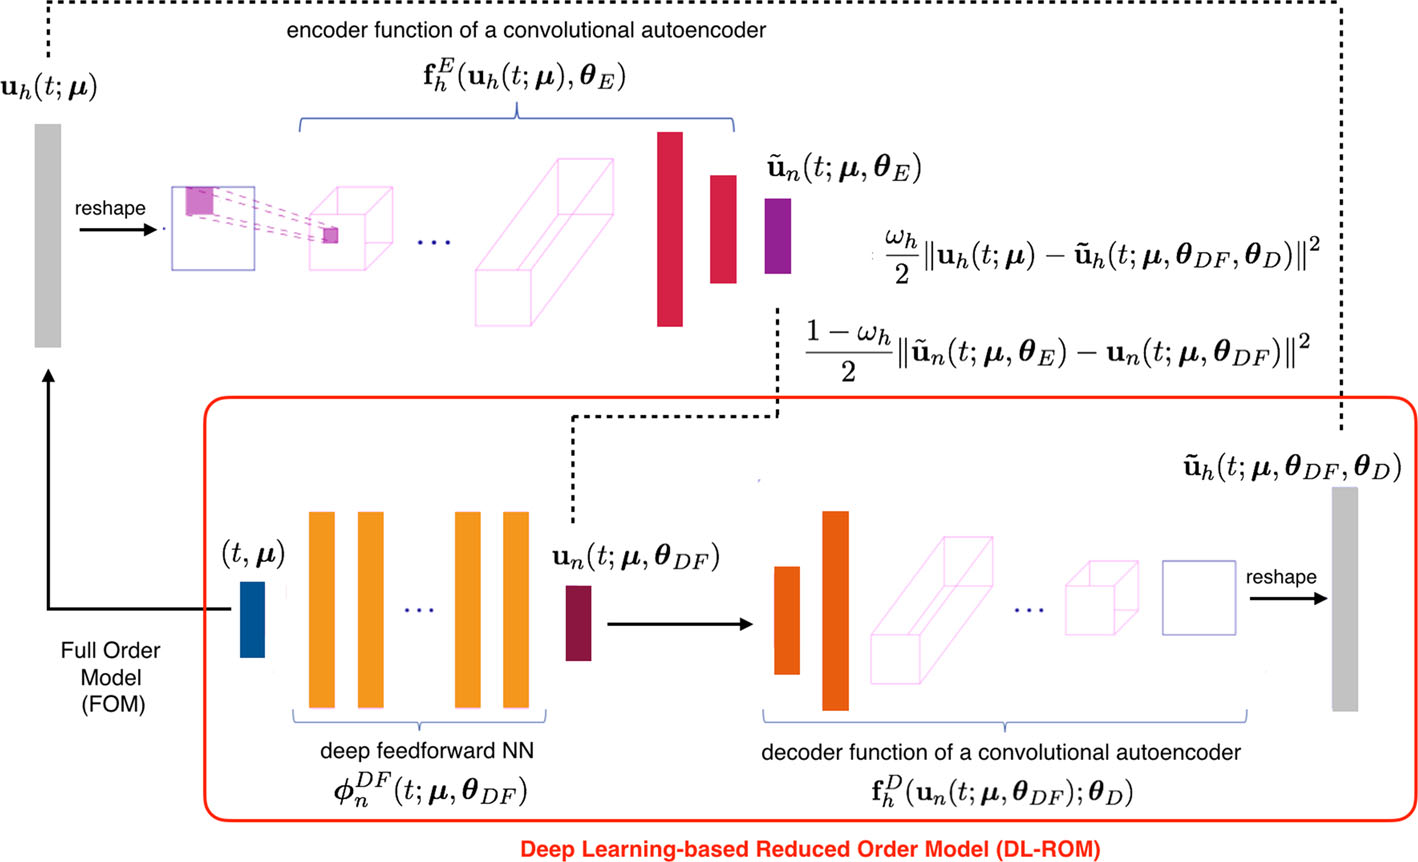
\includegraphics[width=0.8\textwidth]{imgs/dlrom-arch.png}
    \caption{Architecture used for DL-ROM. In the red rectangle the part used during the online stage.}
    \label{fig:dlrom-arch-org}
\end{figure}

The idea behind DL-ROM is very straight forward: approximate both $\Psi$ and $\varphi$ by means of neural networks. The key point is that the intrinsic coordinates $\mathbf u_n$ are not known, thus is not possible to use directly a fully supervised setup. Indeed, the insight is to employ a semi-supervised approach, in which the low dimensional $\mathbf u_n(\boldsymbol \mu)$ is learnt by means of a CAE. Namely, the map $\varphi_n$ is defined as the DFNN $\psi_n^{DF}$ such that
$$\varphi_n: \boldsymbol \mu \mapsto \psi_n^{DF}(\boldsymbol \mu; \boldsymbol \theta^{DF}) = \mathbf u_n(\boldsymbol \mu)$$
where $\boldsymbol \mu \in \mathcal{P}$ are the parameters of the problem and $\boldsymbol  \theta^{DF}$ are the parameters of the network. On the other hand, the map $\Psi_h$ is defined as the decoder part $f_h^D$ of the CAE $f_h^D \circ f_n^E$
$$\Psi_h: \mathbf u_n \mapsto f_h^D(\mathbf u_n; \boldsymbol \theta^D),$$
where $\boldsymbol \theta^D$ are the parameters of the decoder part of the CAE. The DL-ROM approximation is given by combining the two maps together:
$$\boldsymbol \mu \in \mathcal P \mapsto f_h^D(\phi_n^{DF}(\boldsymbol \mu; \boldsymbol \theta^{DF}); \boldsymbol \theta^D)= \tilde{\mathbf u}_h(\boldsymbol \mu) \in \mathbb R^{N_h \times k}.$$
This part of the DL-ROM model (i.e. the online part of the model) is represented in the red box of Figure~\ref{fig:dlrom-arch-org}. The part still missing is how to compute the intrinsic coordinates vector $\mathbf u_n$. As said before, a CAE is exploited to reduce the dimensionality of the input and get the existimate $\tilde{\mathbf u}_n$ of the intrinsic coordinates, namely
$$\mathbf u_h \mapsto f_n^E(\mathbf u_h; \boldsymbol \theta^E) = \tilde{\mathbf u}_n, \quad \mathbf u_h \mapsto f_h^D(f_n^E(\mathbf u_h; \boldsymbol \theta^E); \boldsymbol \theta^D) = \tilde{\mathbf u}_h.$$
Then, one could think of an algorithm in two stages in which 
\begin{enumerate}
    \item Train the CAE $f_h^D \circ f_n^E$ and obtain the parameters $\boldsymbol \theta^E, \boldsymbol \theta^D$. Thus, $\Psi_h = f_h^D(\cdot; \boldsymbol \theta^D)$ and the estimated intrinsic coordinates $\tilde{\mathbf u}_n$ of $\mathbf u_h$ are $\tilde{\mathbf u}_n = f_n^E(\mathbf u_h; \boldsymbol \theta^E)$.
    \item Train the DFNN and obtain $\boldsymbol \theta^{DF}$. Hence, $\varphi_n = \psi_n^{DF}(\cdot; \boldsymbol \theta^{DF})$.
\end{enumerate}
However, \cite{fresca2021comprehensive} has shown that a monolithic approach, where the CAE and DFNN are trained together shows better results both in terms of accuracy and computational cost. Namely, given a dataset of snapshots 
$$\{\boldsymbol \mu^i, \mathbf u_h^i\}_{i=1}^{N_s} \subset \mathcal P \times \mathbb R^{N_h \times k}$$
the training is done by minimizing the objective
$$J(\boldsymbol \theta)=\frac{1}{N_s}\sum_{i=1}^{N_s}\left[\frac{\omega}{2}\mathcal L(\mathbf u_h^i, f^D_h(f^E_n(\mathbf u_h^i; \boldsymbol \theta_E); \boldsymbol \theta_D))+\frac{1-\omega}{2}\mathcal L(f^E_n(\mathbf u_h^i; \boldsymbol \theta_E), \psi_n^{DF}(\boldsymbol \mu^i; \boldsymbol \theta_{DF}))\right],$$
where $\boldsymbol \theta=(\boldsymbol \theta_E, \boldsymbol \theta_D, \boldsymbol \theta_{DF})$, $\mathcal L$ is the loss function (MSE in the original paper) and $\omega \in (0, 1)$ is a loss weight (hyperparameter). Few remarks about the implementation in \cite{fresca2021comprehensive}:
\begin{itemize}
    \item Training is done using ADAM optimizer, ELU activation function and early stopping.
    \item Data is split into train and validation to tune hyperparameters.
    \item Data normalization is used to enhance the training phase; namely data is linearly rescaled into $[0, 1]$ with respect to the minimum and maximum in the dataset.
    \item In order to use the \texttt{Conv2D} layer in the CAE the data in reshaped into a matrix
    \begin{equation}
        \mathbf u_h \in \mathbb R^{N_h} \mapsto \mathbf u_h^R = \texttt{reshape($\mathbf u_h$)} \in \mathbb R^{N_h^{1/2} \times N_h^{1/2}}
    \label{eq:reshape}
    \end{equation}
    if $N_h \neq 4^m, m \in \mathbb N$ then $\mathbf u_h$ is zero-padded. I will use $\mathbf u_h$ and $\mathbf u_h^R$ interchangeably.
\end{itemize}


\subsection{USM-Net}\label{sec:usmnet}
There are two version of USM-Net: PC-USM-Net and UC-USM-Net, where the latter is a generalization of the former. In both cases, they are a model that takes as input the query point $\mathbf x\in\mathbb R^d$ and the parameters $\boldsymbol \mu \in \mathbb R^{N_\mu}$ and output an approximate value of the solution $\mathbf u(\mathbf x;\boldsymbol \mu) \in \mathbb R^k$. They are approximated by a DFNN, denoted by $\mathcal{NN}$.
The difference is that in UC-USM-Net the solution passes through a system parametric coordinates. Namely, a map $\Phi_{\mathcal G}: (\mathbf x, \boldsymbol \mu) \in \Omega_\mu \times \mathcal P \mapsto \boldsymbol \xi \in \hat\Omega$ that maps a point $\mathbf x \in \Omega_\mu$ to a parametric coordinate $\boldsymbol \xi \in \hat\Omega=[0, 1]^d$ (usually $\hat\Omega=[0, 1]^d$). Figure~\ref{fig:usm-architecture} show a representation of USM-Net. More precisely:
\begin{equation}
    \mathbf u(\mathbf x;\boldsymbol \mu)\approx \mathcal{NN}(\Phi_{\mathcal G}(\mathbf x, \boldsymbol \mu), \boldsymbol \mu; \boldsymbol \theta)
\label{eq:usm-net}
\end{equation}
where $\boldsymbol \theta$ is the set of parameters of the DFNN. Notice that Eq.~\ref{eq:usm-net} holds for both the PC-USM-Net and UC-USM-Net, indeed in the former $\Phi_{\mathcal G}$ is the identity. The insight behind UC-USM-Net is that in the physical space the same point $\mathbf x \in \mathbb R^d$ could be a boundary point, an internal point or an external point for $\Omega_\mu$, depending on $\boldsymbol \mu$. Therefore, the mapping $\Phi_{\mathcal G}$ offers a more effective correspondence between points among geometries. 

The training is done in the following way. Suppose that $N_s$ snapshots of dimension $\{N_h^i\}_{i=1}^{N_s}$ are given:
$$\{\boldsymbol \mu^i,\{\mathbf x^i, \boldsymbol \xi^i, \mathbf u(\mathbf x^i_j;\boldsymbol \mu^i)\}_{j=1}^{N_h^i}\}_{i=1}^{N_s}.$$
Notice that the assumption of having snapshots of different dimension can be really useful since it means that data can come from both physical measurements and numerical experiments. 
Let me stress that the assumption to have also the coordinates in parameter space $\boldsymbol \xi^i$ is not restrictive. Indeed, in most cases $\Phi_{\mathcal G}$ is known a-priori and thus $\boldsymbol \xi^i$ can be pre-computed. Moreover, in other cases, like for instance with NURBS, $\Phi_{\mathcal G}$ is not known but $\boldsymbol \xi^i$ are given by construction. Then, I unroll the snapshots, so to have the following dataset
$$\{\boldsymbol \xi^i, \mathbf x^i, \boldsymbol \mu^i, \mathbf u^i\}_{i=1}^{N_t=\sum_{i=1}^{N_s}N_h^i}$$
where $\mathbf u^i = \mathbf u(\mathbf x^i; \boldsymbol \mu^i)$. Training the USM-Net means to minimize the following objective
\begin{equation}
   J(\theta) = \frac{1}{N_t}\sum_{i = 1}^{N_t} \mathcal L(\mathbf u^i, \mathcal{NN}(\Phi_{\mathcal G}(\mathbf x^i, \boldsymbol \mu^i), \boldsymbol \mu^i; \boldsymbol \theta)) + \mathcal R(\boldsymbol \theta)
\label{eq:usm-obj}
\end{equation}
where $\mathcal L$ is the loss function - usually MSE or MAE or Hubert loss - and $\mathcal R$ is a regularization term such as Tikhonov or LASSO regularization or even a physic-informed residual \cite{raissi2019physics}. Few remarks about the implementation:
\begin{itemize}
    \item When using physic-informed regularization, it must be possible to differentiate $\Phi_{\mathcal G}$, since physic informed neural networks (PINNs) relies on computing the gradient $\nabla_{\mathbf x} \mathcal{NN}$ with automatic differentiation. On the other hand, when not using physic-informed regularization, $\Phi_{\mathcal G}(\mathbf x^i, \boldsymbol \mu^i)$ can be substituted with the pre-computed $\boldsymbol \xi^i$.
    \item Physical constraints can be also enforced in hard form \cite{lu2021physics}. For instance, homogeneous Dirichlet boundary conditions can be applied by multiplication by a mask function.
    \item The dataset is split into training/validation/test and the objective \ref{eq:usm-obj} is minimized with samples only from the training dataset.
\end{itemize}


\subsection{NURBS}
Discretization methods - like finite elements and finite volumes - assemble on the elements of the mesh a suitable approximation of the operators associated with the PDE. Unfortunately, changes in shape of the domain require the re-execution of the entire process, necessitating the reallocation of significant computational resources.
For this reason, some computational approaches, like
Isogeometric Analysis (IGA) and shape models, are designed to avoid the regeneration of a new computational mesh when a change of geometry occurs.
IGA achieves this thanks to the use of non-uniform rational B-splines (NURBS) \cite{piegl1996nurbs} that exactly match CAD geometries, usually adopted in an industrial context \cite{hughes2005isogeometric}.

The key aspect of a NURBS surface that I will leverage in this manuscript is that they work as a geometrical mapping $\Phi_{\mathcal G}: \boldsymbol \xi \in [0, 1]^2 \mapsto \mathbf x \in \mathbb R^d, d=2,3$ from a parametric space to the physical space.

\section{Numerical Results}\label{sec:numericres}
In this section I report the results I obtained by applying the two DL-based ROM techniques introduced in the previous section. Namely, I will apply them to two model problems, where the data is obtained by the means of IGA through the GeoPDEs library \cite{vazquez2016new}. Let me now explain how I apply these two techniques.
\begin{itemize}
\item I apply the DL-ROM approach introduced in the Section~\ref{sec:dlrom} with a small modification. Namely, in order to have a computationally cheaper model, I have cut away the encoder part of the autoencoder (thus also removed the loss part concerning $\mathbf u_n(\boldsymbol\mu)$ and $\tilde{\mathbf u}_n(\boldsymbol\mu)$). The resulting architecture is shown is Figure~\ref{fig:dlrom-architecture}. Indeed, I expect the decoder function to implicitly learn the intrinsic coordinates $\mathbf u_n(\boldsymbol\mu)$. 

An advantage of using FOM derived from IGA is that it is trivial to directly obtain a solution $\mathbf u_h^R \in \mathbb R^{N_h^{1/2}\times N_h^{1/2}}$ (see Eq.~\ref{eq:reshape}). Indeed, it is enough to evaluate the solution $\mathbf u_h$ at the parametric points of the form $\boldsymbol \xi = (m_1/M_1, m_2/M_2)$ where $m_i = 0, ..., M_i, \, M_i \in \mathbb N, \, i=1,2$ define an uniform sampling of $[0, 1]$.
\item I apply both PC-USM-Net and UC-USM-Net exactly how I introduced them in Section~\ref{sec:usmnet}. However, in the original paper, the authors rely on
a Laplacian-based field $\Phi_{\mathcal G}$ to pass from the physical space to the parametric space. In my case this is not needed since the coordinates in the parametric space are known when resolving a PDE with IGA. Then, it is possible to approximate the map $\Phi_{\mathcal G}$ by the means of a neural network. The representation of the architecture for PC-USM-Net and UC-USM-Net is shown in Figure~\ref{fig:usm-architecture}, where, in the latter case, there is an extra loss for the approximation of $\Phi_{\mathcal G}$ by means of a DFNN. 
\end{itemize}

To evaluate the error I will rely on a MSE loss function and the following two error metric
$$l^p = \left(\sum_{i=0}^{N_t}|\mathbf u(\mathbf x^i; \boldsymbol \mu^i) - \tilde{\mathbf u}(\mathbf x^i; \boldsymbol \mu^i)|^p / N_t\right)^{1/p},\quad p=1,2.$$
Notice that this metric can be applied to the DL-ROM since, by definition, $\mathbf u_h(\boldsymbol \mu)=\mathbf u(\mathbf x^i; \boldsymbol \mu)$ for a fixed set of $\{\mathbf x^i\}_{i=1}^{N_h} \subset \mathbb R^d$.
Moreover, in the case of DL-ROM, I employ the following metric
\begin{equation}
\epsilon = \frac{1}{N_t} \sum_{i=0}^{N_t}\sqrt{\frac{||\mathbf u_h(\boldsymbol \mu^i) - \tilde{\mathbf u}_h(\boldsymbol \mu_i)||_2^2}{||\mathbf u_h(\boldsymbol \mu^i)||_2^2}}
    \label{eq:err_metric}
\end{equation}
If not stated otherwise I use ADAM optimizer with default starting learning rate of 1e-3 and batch size of 32. Moreover, I will always employ a learning rate scheduler to reduce the gradient step on plateaus. With abuse of notation, I assume the training dataset is made by $N_t$ randomly chosen samples from the original dataset. 

Finally, let me mention that DL-ROM and USM-Net training was carried out on different machines, so training time in not directly comparable among the two. As rule of thumb, multiply the DL-ROM training time by a factor of 2.5 to compare it to USM-Nets.

\begin{figure}[t]
    \centering
    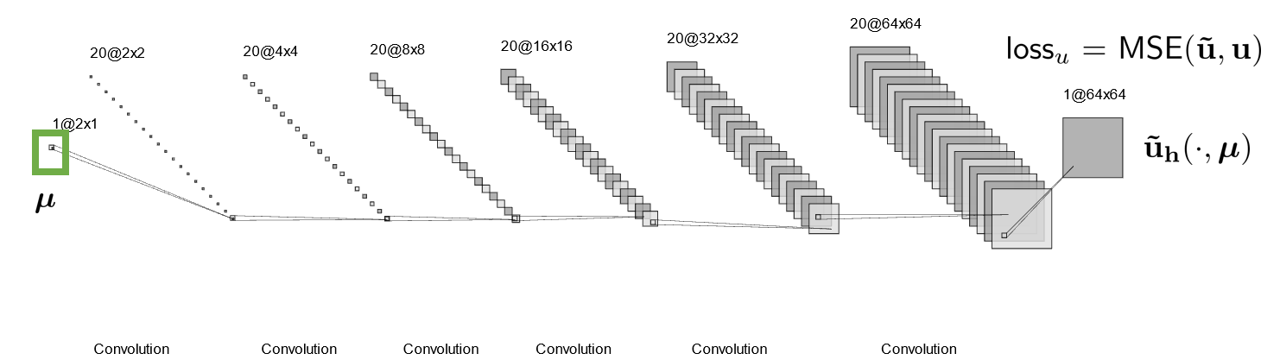
\includegraphics[width=\textwidth]{imgs/dl-rom.png}
    \caption{Architecture used for DL-ROM}
    \label{fig:dlrom-architecture}
\end{figure}

\begin{figure}[t]
    \centering
    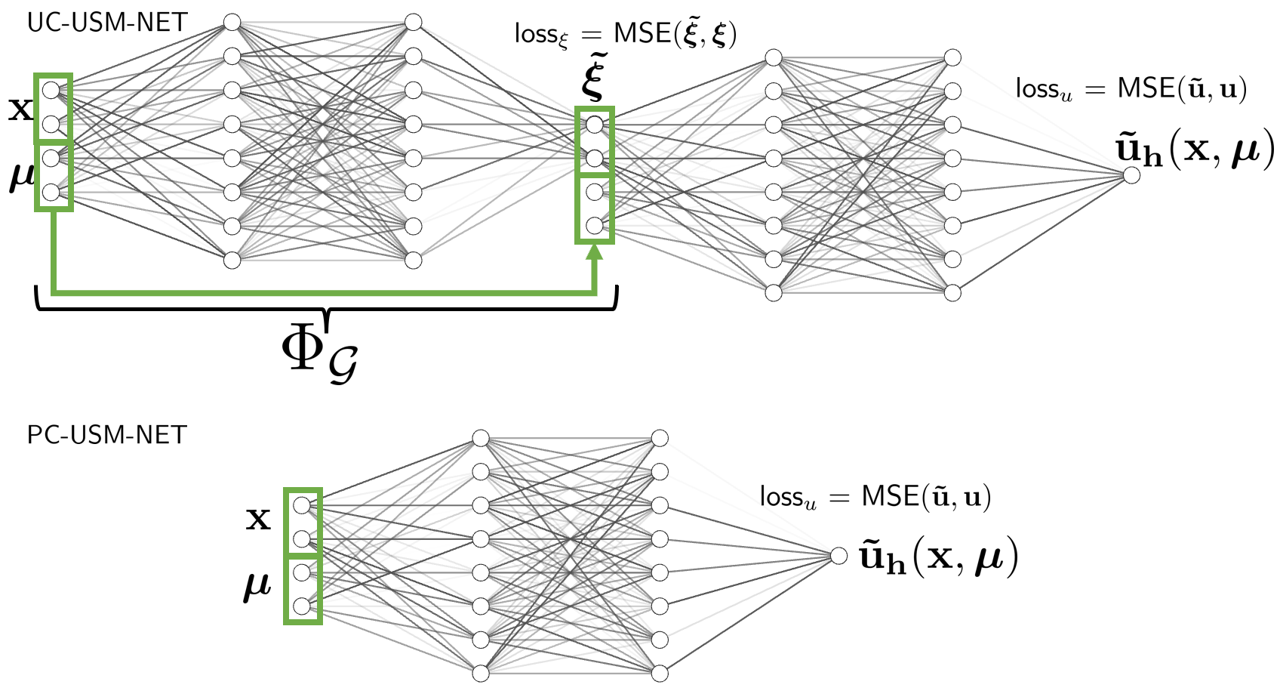
\includegraphics[width=\textwidth]{imgs/usm-net.png}
    \caption{Architecture used for USM-Net}
    \label{fig:usm-architecture}
\end{figure}


\subsection{Test Case 1: Poisson's equations}
In this test case I solve the following (scalar) Poisson equation in the domain $\Omega$ shown a in Figure~\ref{fig:quarterring}.

\begin{equation}
    \begin{cases}
    -\Delta \mathbf u = 1 & \textnormal{ in } \Omega\\
    \mathbf u = 0 & \textnormal{ on } \partial\Omega_D\\
    \partial_n \mathbf u = 0 & \textnormal{ on } \partial\Omega_N\\
    \end{cases}
\label{eq:problem1}
\end{equation}

Namely $\Omega$ is described by a NURBS with all weights equal to one and the following nodes and control points (which depend on the scalar parameters $(\boldsymbol \mu)_1, (\boldsymbol \mu)_2 \in \mathbb R^+$)
\begin{equation*}
    \Xi_1 = \{0, 0, 0, 1, 1, 1\}, \quad
    \Xi_2 = \{0, 0, 1, 1\}, \quad
    P_i \in \bigg\{
\begin{bmatrix}
     1\\0
\end{bmatrix},
\begin{bmatrix}
     (\boldsymbol \mu)_1\\(\boldsymbol \mu)_1
\end{bmatrix}, 
\begin{bmatrix}
     0\\1
\end{bmatrix}, 
\begin{bmatrix}
     2\\0
\end{bmatrix}, 
\begin{bmatrix}
     (\boldsymbol \mu)_2\\ (\boldsymbol \mu)_2
\end{bmatrix} ,
\begin{bmatrix}
     0\\2
\end{bmatrix} 
    \bigg\}    
\end{equation*}


\begin{figure}[t]
\centering
\begin{minipage}{.4\textwidth}
    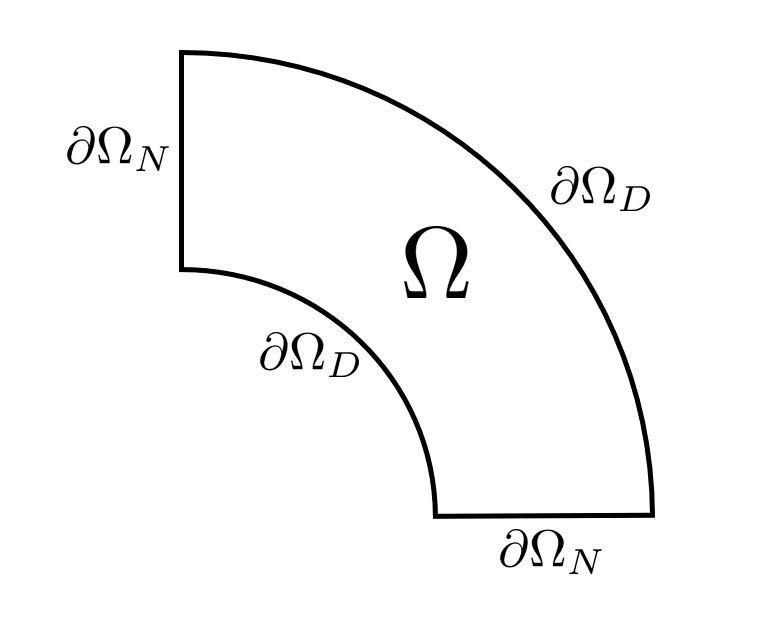
\includegraphics[width=\textwidth]{imgs/quarter-ring.png}
    \caption{Undeformed quarter ring domain $\Omega_{\boldsymbol \mu=((\boldsymbol \mu)_1, (\boldsymbol \mu)_2)=(1, 2)}$ of Problem~\ref{eq:problem1} }
    \label{fig:quarterring}
\end{minipage}%
\hfill
\begin{minipage}{.59\textwidth}
    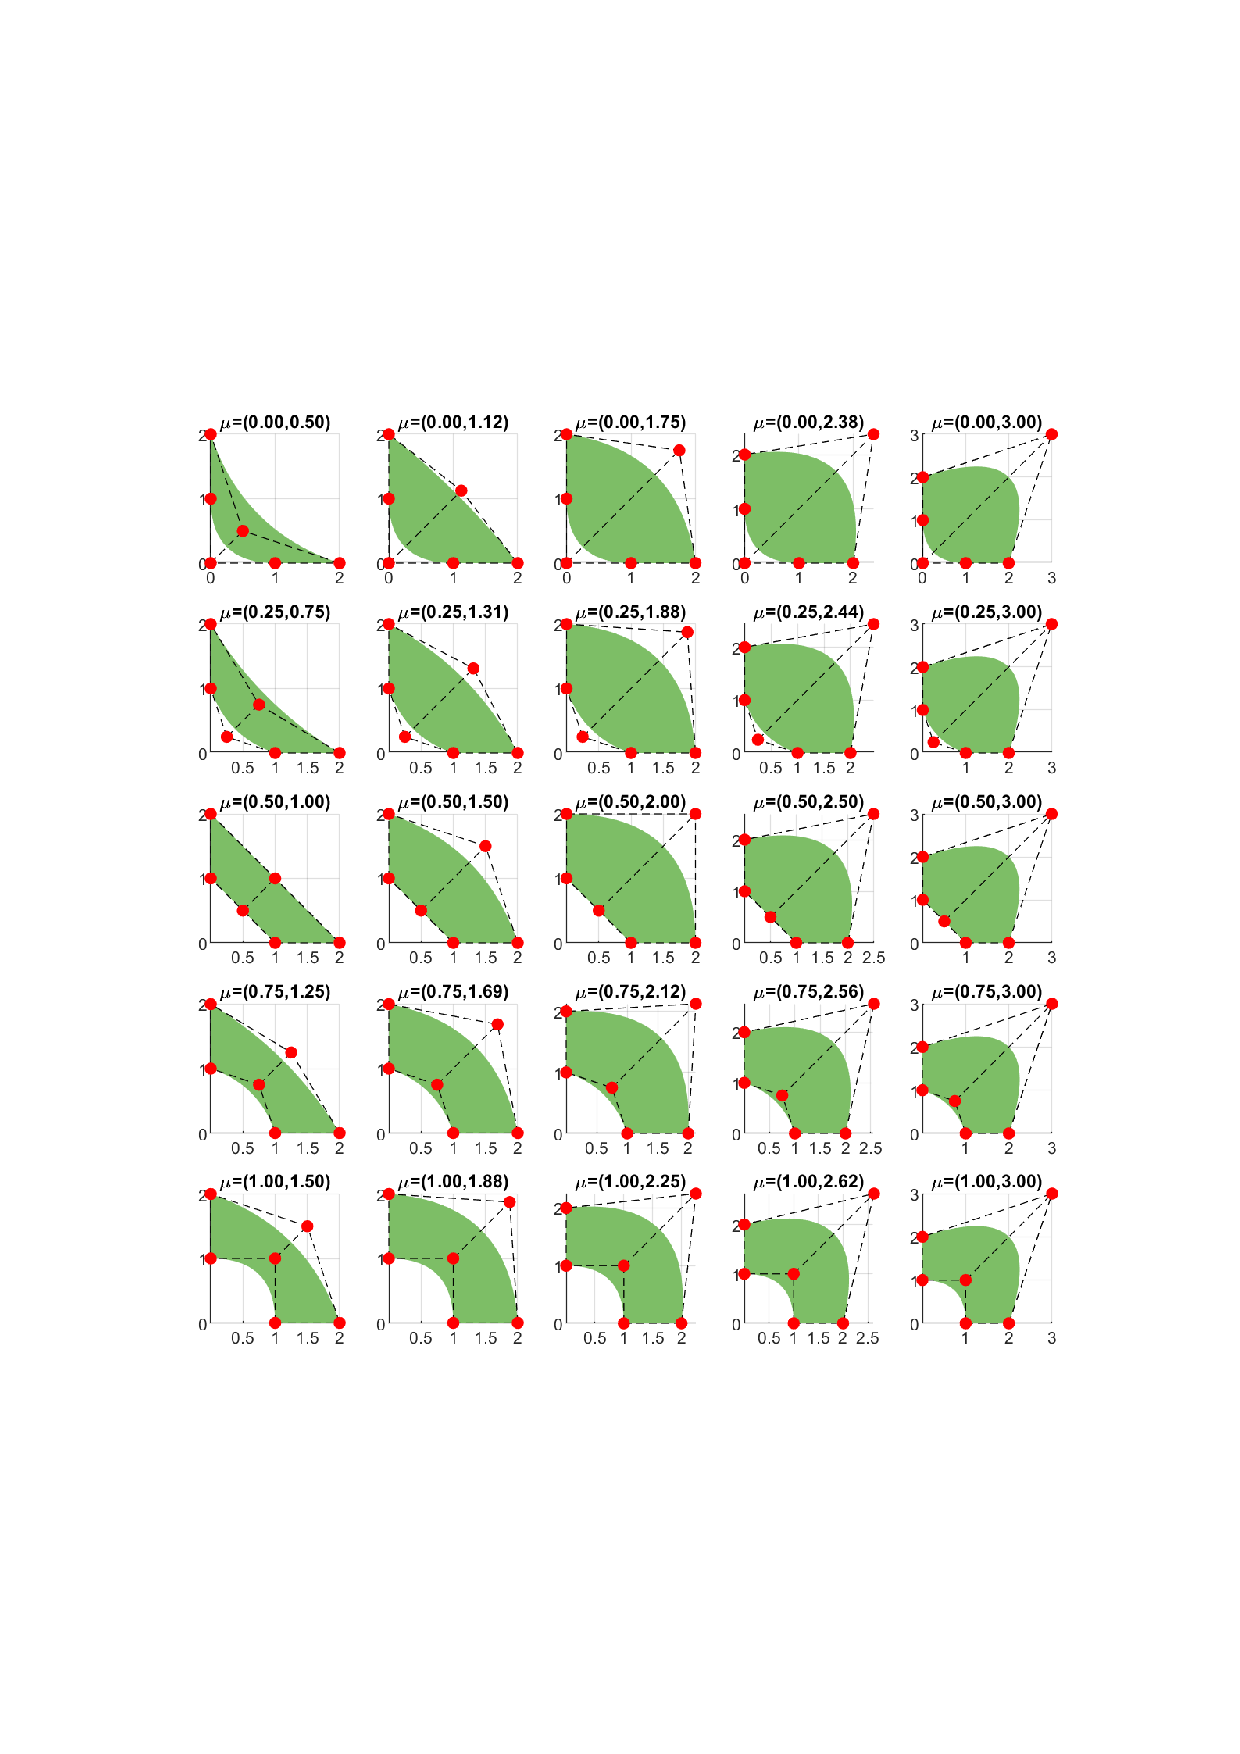
\includegraphics[trim={3.3cm 6.5cm 3cm 7cm},clip,width=\textwidth]{imgs/quarter-ring-deform.pdf}
    \caption{Domain $\Omega_{\boldsymbol \mu}$ of Eq.~\ref{eq:problem1} for some choices of the parameters $\boldsymbol \mu$.}
    \label{fig:quarer-ring-def}
\end{minipage}
\end{figure}

\begin{figure}[t]
    \centering
    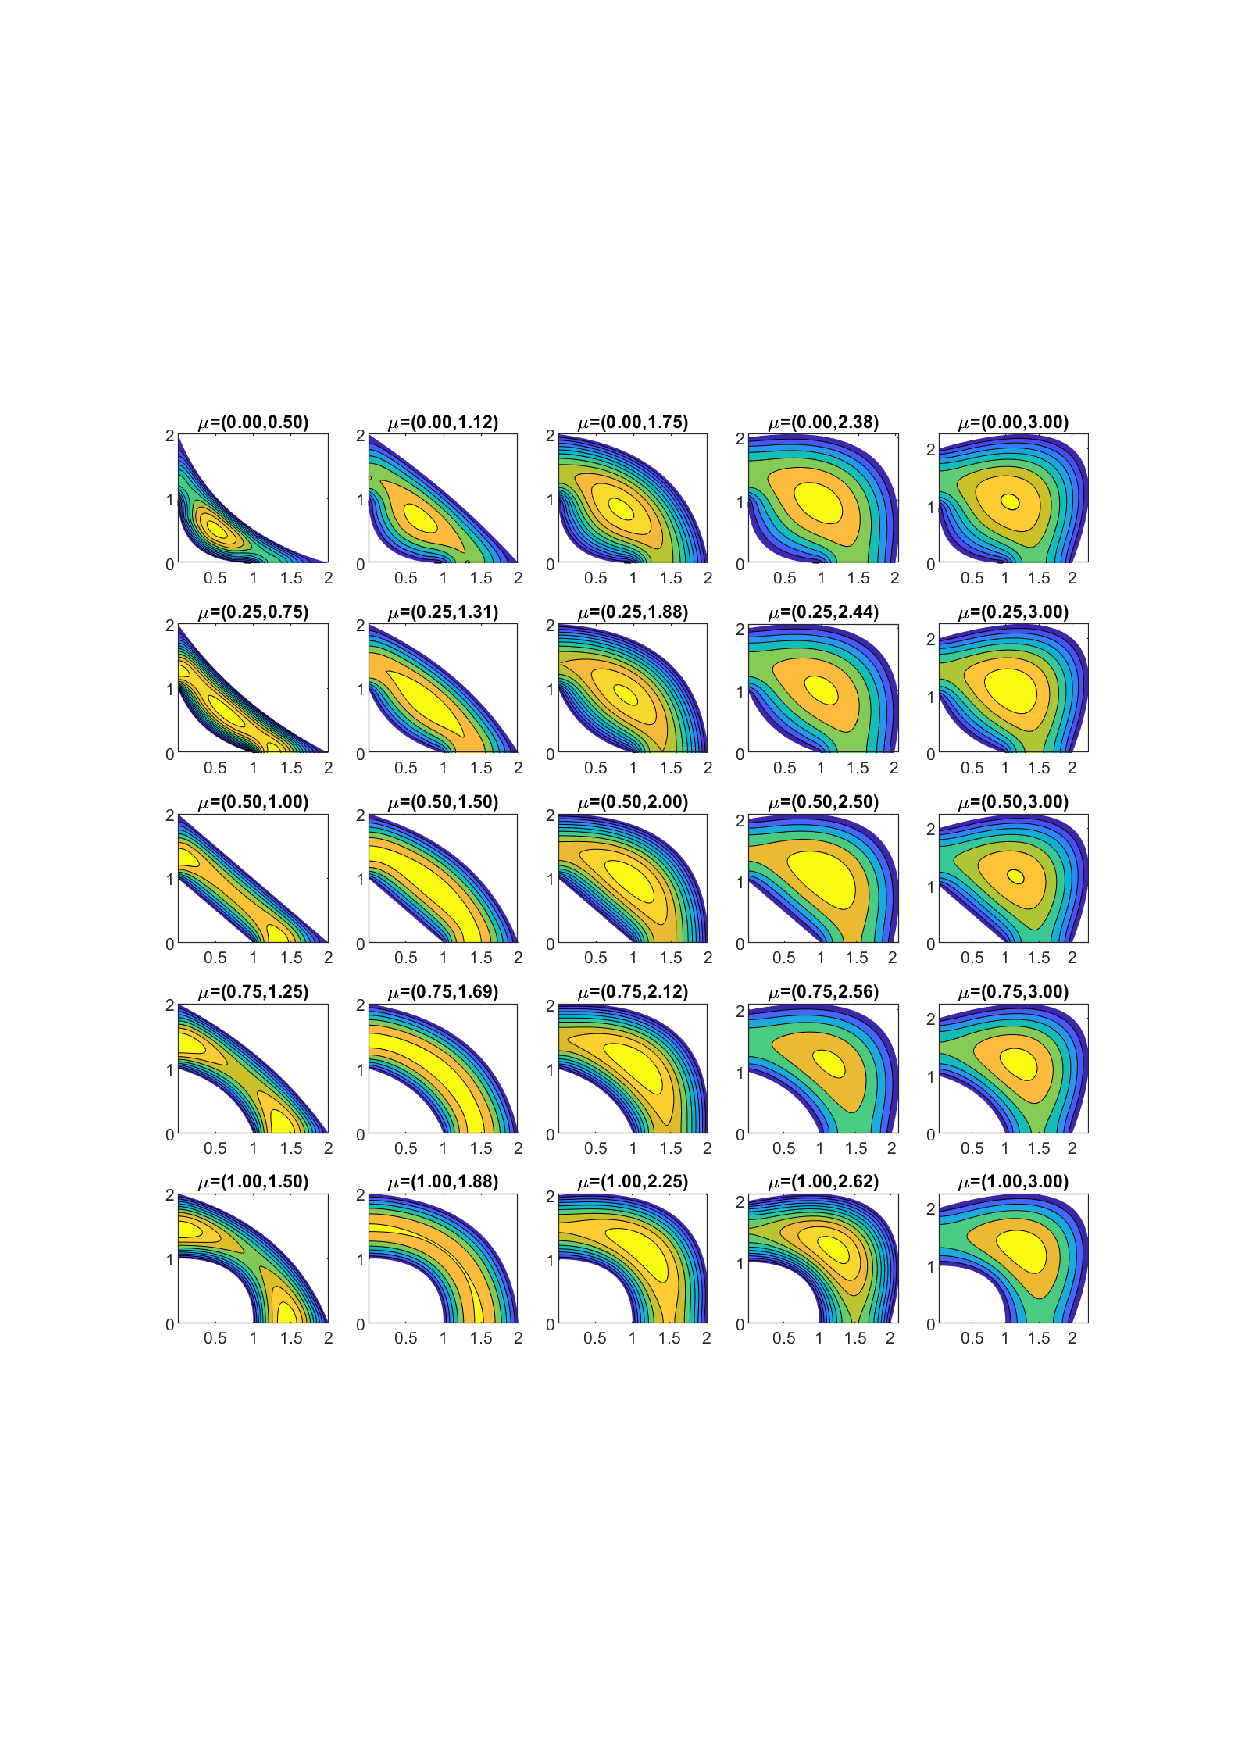
\includegraphics[trim={2.7cm 6.5cm 2cm 7cm},clip,width=.7\textwidth]{imgs/quarter-ring-deform-solved.pdf}
    \caption{Solution of Eq.~\ref{eq:problem1} on some domains $\Omega_{\boldsymbol \mu}$}
    \label{fig:quarer-ring-def-sol}
\end{figure}


The geometry of the domain $\Omega$ is modified by moving the position of two control points (i.e.\ by varying $\boldsymbol \mu$) along the bisector of the first quadrant. Figure~\ref{fig:quarer-ring-def} shows some of the resulting geometries. Figure~\ref{fig:quarer-ring-def-sol} shows the solution of the PDE computed in the same domains of Figure~\ref{fig:quarer-ring-def} after applying $h$-refinement and $p$-refinement. The dataset is generated by sampling uniformly 15 values of $(\boldsymbol \mu)_1$ in $[0, 1]$, 15 values of $(\boldsymbol \mu)_2$ in $[(\boldsymbol \mu)_1, 3]$, and 127 values of each component of coordinates in parametric space $(\boldsymbol \xi)_i, i=1,2$. 

\subsubsection{DL-ROM}\label{sec:dlrom-lapl}
The dataset contains $15^2$ spatially subsampled FOM solutions $\mathbf u_h \in \mathbb R^{64 \times 64}$ with respective parameters $\boldsymbol \mu$. The architecture of the model is shown in Figure \ref{fig:dlrom-architecture}. As in the original paper, I employ a 80-20 train-validation splitting. First I test different activation functions.

\begin{center}
\begin{tabular}{ c|c|c|c|c|c|c|c } 
 $N_t$ & filters & kernel size & activation & train time [s] & $l^1$ & $l^2$ & $\epsilon$ \\ 
 \hline
 180 & 32 & 5 & ReLU & 45.55 &  1.21e-3 & 1.65e-3   & 1.43e-2\\
 180 & 32 & 5 & SELU &  45.67 &  2.14e-3 & 3.07e-3  & 2.80e-2\\
 180 & 32 & 5 & ELU &  45.45 &  5.35e-3 & 7.26e-3   & 6.48e-2\\
 180 & 32 & 5 & PReLU &  46.10 &  1.21e-3 & 1.88e-3 & 1.63e-2\\
\end{tabular}
\end{center}
ReLU and PReLU seem to lead to the lowest test metric. Moreover, PReLU has comarable computational cost to ReLU even if the model has more parameters. Using PReLU as activation  I tune the kernel size and number of filters. The following table shows the $l^2$ metric.

\begin{center}
\begin{tabular}{ l||c| c |c |c |c } 
   kernel size  & 3 & 4 & 5 & 6 & 7 \\ 
   filters &  &  &  &  &  \\ 
 \hline
 \hline
 16 & 4.51e-3 & 2.66e-3 & 1.99e-3 & 2.22e-3 & 2.25e-3 \\
 \hline
 24 & 2.29e-3 & 1.91e-3 & 2.29e-3 & 1.84e-3 & 1.35e-3  \\
 \hline
 32 & 1.90e-3 & 1.77e-3 & 1.84e-3 & 1.81e-3 & 1.53e-3  \\
 \hline
 40 & 1.67e-3 & 1.77e-3 & 1.43e-3 & 1.47e-3 & 1.67e-3  \\
 \hline
 48 & 1.91e-3 & 1.42e-3 & 1.32e-3 & 1.31e-3 & 1.25e-3  \\
 \hline
 64 & 1.37e-3 & 1.21e-3 & 1.54e-3 & 1.29e-3 & 1.66e-3 \\
\end{tabular}
\end{center}

I now compare ReLU and PReLU for the filters and kernel sizes that obtained the lowest test metric.

\begin{center}
\begin{tabular}{ |c|c|c|c|c|c|c|c|c|c| } 
 &&kernel&avg train&\multicolumn{3}{c|}{ReLU}&\multicolumn{3}{c|}{PReLU}\\
 $N_t$ & filters & size  &  time [s] & $l^1$ & $l^2$ & $\epsilon$ & $l^1$ & $l^2$ & $\epsilon$ \\ 
 \hline
 180 & 64 & 4 & 88.45 & 8.23e-4 & 1.17e-3 & 1.07e-2 & 1.14e-3 & 1.69e-3 & 1.48e-2\\
 180 & 64 & 6 & 166.47 & 7.76e-4 & 1.16e-3 & 1.03e-2 & 6.59e-4 & 1.02e-3 & 8.98e-3\\
 180 & 64 & 7 & 194.98 & 6.29e-4 & 9.68e-4 & 8.79e-3 & 7.15e-4 & 1.09e-3 & 9.86e-3\\
 180 & 48 & 5 & 100.76 & 9.57e-4 & 1.40e-3 & 1.23e-2 & 1.00e-3 & 1.58e-3 & 1.37e-2\\
 180 & 48 & 7 & 147.52 & 7.42e-4 & 1.11e-3 & 9.80e-3 & 8.28e-4 & 1.40e-3 & 1.21e-2\\
\end{tabular}
\end{center}

ReLU seems to give the better results, moreover, considering it is less expensive I choose ReLU for this final test. Namely, I increase the maximum number of epochs to 800 and train the two best models. These are the results.

\begin{center}
\begin{tabular}{ c|c|c|c|c|c|c|c } 
 $N_t$ & filters & kernel size & activation & train time [s] & $l^1$ & $l^2$ & $\epsilon$ \\ 
 \hline
 180 & 48 & 7 & ReLU & 216.29 & 5.49e-4 & 8.03e-4 & 7.25e-3\\
 180 & 64 & 7 & ReLU & 299.34 & 6.25e-4 & 9.23e-4 & 8.30e-3\\

\end{tabular}
\end{center}
I have also tested different sizes for the mini-batch (64, 128) but results were always worse.


\subsubsection{USM-Net}\label{sec:usmnet-lapl}
The unrolled dataset totals 3~629~025 data samples. I start by using a UC-USM-Net with input the parametric coordinates $\boldsymbol \xi$. I employ a DFNN with $l$ layers of width $w$, for short $l \times w$ (i.e.\ the architecture is the one of the PC-USM-Net in Figure \ref{fig:usm-architecture} bottom). First I test different activation functions.

\begin{center}
\begin{tabular}{ c|c|c|c|c|c } 
 $N_t$ & size & activation & train time [s] & $l^1$ & $l^2$ \\ 
 \hline
 2e4 & $8\times 80$ & ELU & 275.00 &  3.35e-4 & 5.13e-4\\
 2e4 & $8\times 80$ & ReLU & 263.82 & 6.48e-4 & 9.72e-4\\
 2e4 & $8\times 80$ & SELU & 271.01 &  6.57e-4 & 9.48e-4 \\
 2e4 & $8\times 80$ & PReLU & 324.95 &  4.81e-4 & 7.53e-4 \\
 2e4 & $8\times 80$ & Tanh & 256.99 &  5.07e-4 & 8.44e-4 \\
\end{tabular}
\end{center}

I notice that ELU leads to the lowest loss and Tanh has the lowest computational cost. It is reasonable that a function with continuous derivative gives the best results in the context of a DFNN. It follows a study of the size of the model.

\begin{center}
\begin{tabular}{ c|c|c|c|c|c|c } 
 $N_t$ & size & avg train time [s] & ELU $l^1$ & ELU $l^2$ & Tanh $l^1$ & Tanh $l^2$ \\ 
 \hline
 2e4 & $6\times 60$ & 217.73 & 4.82e-4 & 7.67e-4 & 6.58e-4 & 1.14e-3\\
 2e4 & $7\times 70$ & 241.14 & 4.23e-4 & 7.01e-4 & 4.11e-4 & 6.81e-4\\
 2e4 & $8\times 80$ & 267.01 & 3.01e-4 & 4.89e-4 & 4.38e-4 & 7.22e-4 \\
 2e4 & $9\times 90$ & 305.25 & 3.24e-4 & 5.20e-4 & 4.11e-4 & 6.89e-4 \\
\end{tabular}
\end{center}

The optimal size seems to stay in a neighborhood of $8\times 80$, a larger size seems to lead to lower performances, this could be due to the fact that deeper models are harder to train. Then I study the impact of the size of the training dataset
\begin{center}
\begin{tabular}{ c|c|c|c|c|c } 
 $N_t$ & size & activation & train time [s] & $l^1$ & $l^2$ \\ 
 \hline
 1e4 & $8\times 80$ & Tanh & 133.62 &  1.25e-3 & 1.73e-3\\
 2e4 & $8\times 80$ & Tanh & 256.79 &  4.03e-4 & 6.74e-4\\
 4e4 & $8\times 80$ & Tanh & 518.58 &  2.72e-4 & 3.99e-4\\
 8e4 & $8\times 80$ & Tanh & 1019.67 &  2.00e-4 & 3.18e-4\\
 16e4 & $8\times 80$ & Tanh & 2067.68 &  1.35e-4 & 2.07e-4\\
\end{tabular}
\end{center}
Larger sizes of the training dataset is really beneficial but it also increases the computational cost consistently. Due to the large computational cost I am always using a very small percentage of the full dataset for training ($\sim 1\%$), but at the same time I am obtaining very good results with respect to the test metrics. Figure~\ref{fig:usmnet-trained} shows an example of a trained model. I repeat some of the same experiments for a PC-USM-Net. Namely, the overall architecture is the same as before but I use as inputs the physical coordinates.

\begin{center}
\begin{tabular}{ c|c|c|c|c|c|c } 
 $N_t$ & size & avg train time [s] & ELU $l^1$ & ELU $l^2$ & Tanh $l^1$ & Tanh $l^2$ \\ 
 \hline
 2e4 & $6\times 60$ & 228.98 & 3.94e-4 & 6.15e-4 & 3.81e-4 & 6.71e-4\\
 2e4 & $7\times 70$ & 246.07 & 3.82e-4 & 6.24e-4 & 3.11e-4 & 5.15e-4\\
 2e4 & $8\times 80$ & 270.06 & 3.61e-4 & 4.96e-4 & 3.14e-4 & 5.44e-4\\
\end{tabular}
\end{center}

As expected from the results in \cite{regazzoni2022}, employing the physical coordinates lead to a more difficult training and a slightly larger loss with respect to the parametric coordinates. Finally, I carry out some experiments for a UC-USM-Net with a learned $\Psi_{\mathcal G}$. Namely, I use the architecture in Figure \ref{fig:usm-architecture} top: the input are the physical coordinates and at the same time the model learns the physical to parametric mapping thanks to a secondary loss.

\begin{center}
\begin{tabular}{ |c|c|c|c|c|c|c|c|c| } 
 $N_t$ & size $\Psi_G$ & size head & activation & train time [s] & $l^1$ & $l^2$ & $l^2$ $\Psi_G$\\ 
 \hline
 2e4 & $6\times 60$ & $6\times 60$ & Tanh & 331.65 & 5.21e-4 & 8.33e-4 & 1.05e-3\\
 2e4 & $7\times 70$ & $7\times 70$ & Tanh & 380.78 & 3.63e-4 & 5.85e-4 & 7.31e-4\\
 2e4 & $7\times 70$ & $8\times 80$ & Tanh & 402.05 & 5.09e-4 & 7.17e-4 & 9.38e-4\\
\end{tabular}
\end{center}
The model succeed in learning $\Psi_{\mathcal G}$, however the training is more computationally expensive. Results are comparable (if not slightly better) with PC-USM-Net. The advantage of this approach for UC-USM-Net with respect to using the precomputed $\boldsymbol \xi$ as inputs (i.e.\ the model proposed at the start of this section) is that it is possible to use a PINN-like term in the regularizer part of the loss. 

\begin{figure}[t]
    \centering
    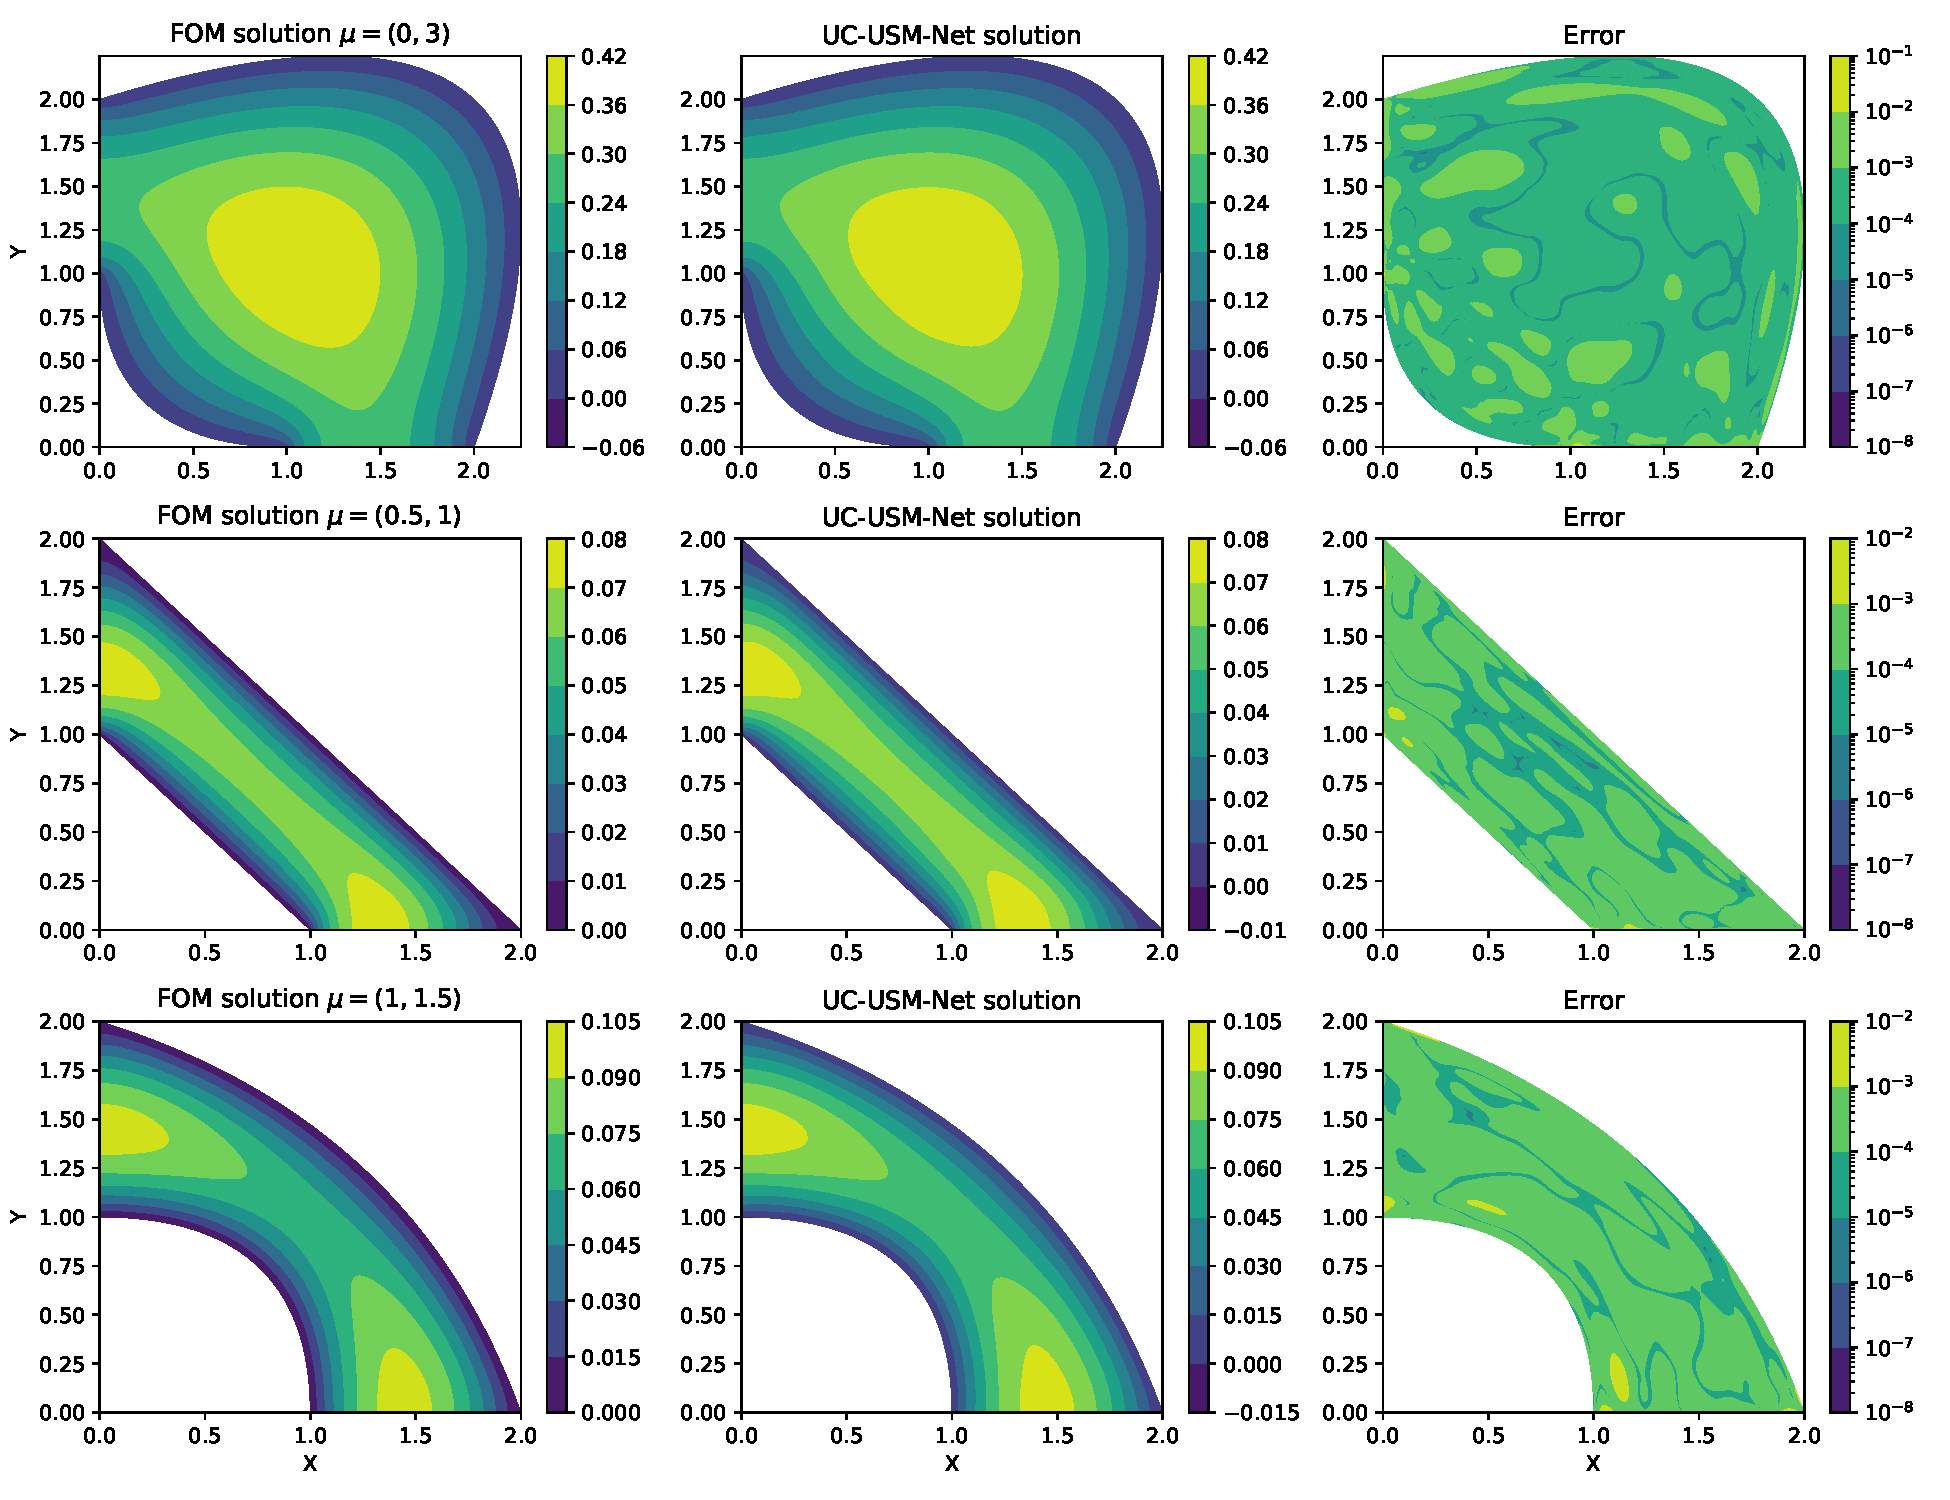
\includegraphics[width=0.8\textwidth]{imgs/lapl_pinn_trained.pdf}
    \caption{Example of trained UC-USM-Net for some choices of $\boldsymbol \mu$. Hyperparams: depth=8, width=80, activation=ELU, $N_t=$4e4, epochs=300.}
    \label{fig:usmnet-trained}
\end{figure}

\subsection{Test Case 2: Scordelis-Lo Roof}
I now consider an elasticity problem defined on a surface (shell) immersed in a 3D domain. I use the Kirchhoff-Love shell theory \cite{kiendl2009isogeometric} to solve the Scordelis-Lo roof benchmark \cite{scordelis1964computer, belytschko1985stress}. Namely, a section of a cylinder (cut with a plane parallel to its axis) is loaded by its own weight and supported on rigid diaphragms at each end with the other two boundaries being free. Figure~\ref{fig:scordelislo-setting} shows a representation of the problem. 


\begin{figure}
\centering
\begin{minipage}{.4\textwidth}
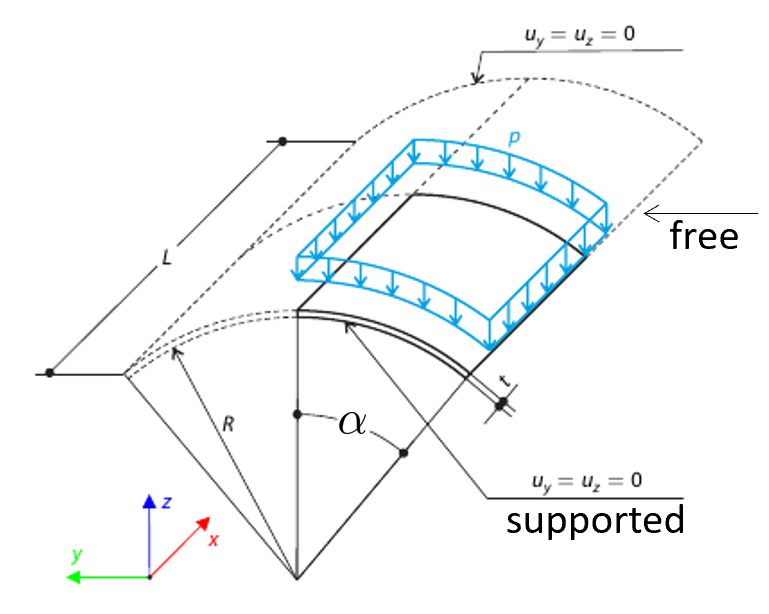
\includegraphics[width=\textwidth]{imgs/scrodelis-lo-roof.png}
    \caption{Schema of the Scordelis-Lo roof benckmark.}
    \label{fig:scordelislo-setting}
\end{minipage}%
\hfill
\begin{minipage}{.58\textwidth}
    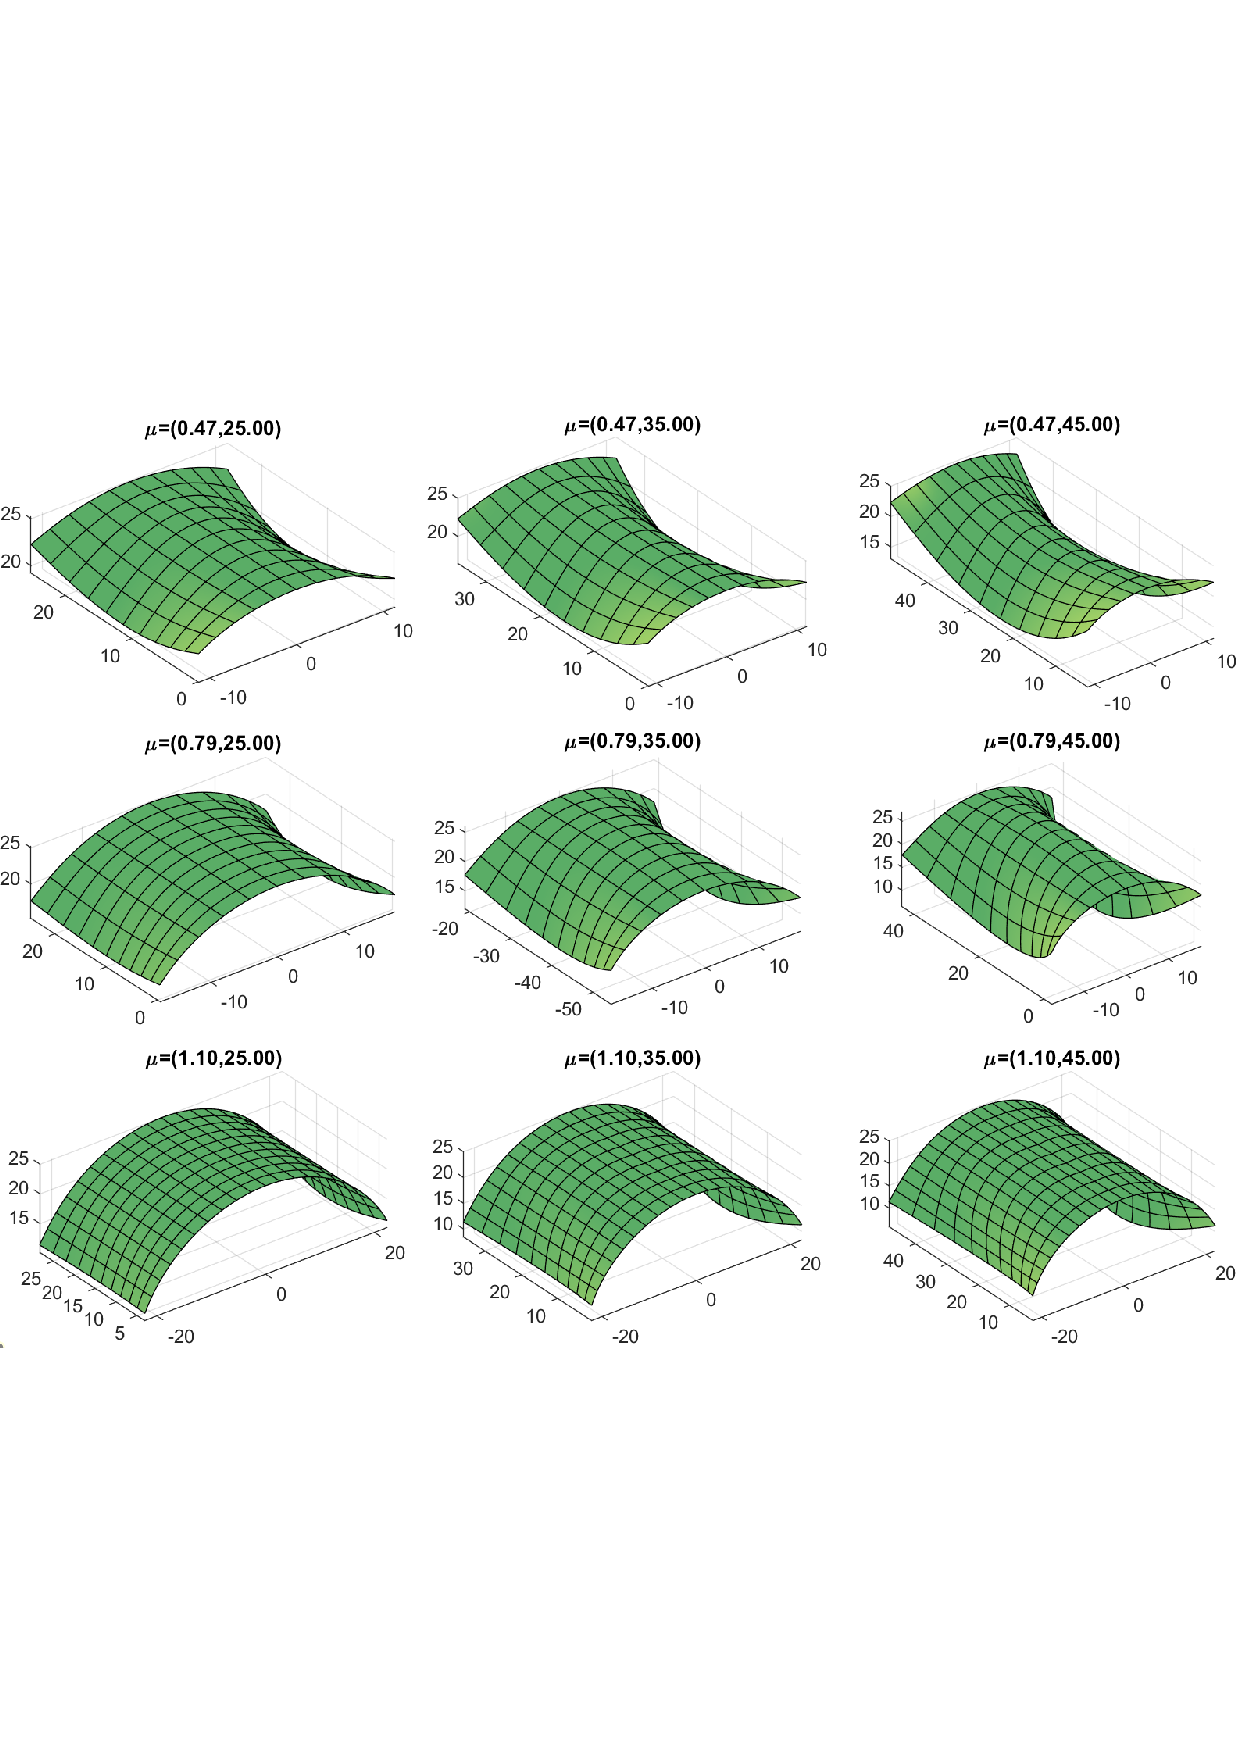
\includegraphics[trim={0 6.5cm 0 7cm},clip,width=\textwidth]{imgs/scrodelis-lo-roof-solved.pdf}
    \caption{Solutions (deformations) of the Scordelis-Lo roof benchmark for some choices of the parameters $\boldsymbol \mu=(\alpha, L)$ applied to the original domain. The deformation in magnified by a factor of 50.}
    \label{fig:scordelislo-sol}
\end{minipage}
\end{figure}


I deform the domain by changing the length $L$ of the cylinder and the central angle $2\alpha$ that subtends the arc cut by the plane, hence, $\boldsymbol \mu = (\alpha, L)$. Figure~\ref{fig:scordelislo-sol} shows some of the solution obtained by changing the parameters $\boldsymbol \mu$. For this test case I linearly rescale the data in the interval $[0, 1]$. I consider 40 uniformly sampled values of $\alpha \in [0.1\pi, 0.4\pi]$ and 50 uniformly sampled values of $L \in [20, 50]$.

\subsubsection{DL-ROM}
The dataset contains 2000 FOM solutions $\mathbf u_h \in \mathbb R^{64 \times 64}$ with respective parameters $\boldsymbol \mu$. To account for the fact it is a vectorial problem, the last layer has three filters instead of one. For the activation function I rely on PReLU and ReLU since they gave the best results in Section \ref{sec:dlrom-lapl}. Since the model is computationally expensive I stop the training at 50 epochs. First, I test if a smaller batch size could accelerate up the training (fixed the number of epochs, the training time will be larger but the aim is to check if increasing the number of gradients updates leads to a smaller loss).

\begin{center}
\begin{tabular}{ |c|c|c|c|c|c|c|c| } 
 &&kernel&&train&\multicolumn{3}{c|}{Batch size 32}\\
 $N_t$ & filters & size  &activation&  time [s] & $l^1$ & $l^2$ & $\epsilon$ \\ 
 \hline
 1600 & 40 & 7 & ReLU & 114.78 & 6.85e-3 & 2.04e-2 & 2.04e-2\\
 1600 & 40 & 7 & PReLU & 124.99 & 1.04e-2 & 2.11e-2 & 2.61e-2\\
 1600 & 64 & 7 & ReLU & 158.99 & 6.85e-3 & 1.67e-2 & 1.63e-2\\
 1600 & 64 & 7 & PReLU & 169.20 & 7.06e-3 & 2.26e-2 & 2.13e-2\\
\end{tabular}
\end{center}

\begin{center}
\begin{tabular}{ |c|c|c|c|c|c|c|c| } 
 &&kernel&&train&\multicolumn{3}{c|}{Batch size 16}\\
 $N_t$ & filters & size  &activation&  time [s] & $l^1$ & $l^2$ & $\epsilon$ \\ 
 \hline
 1600 & 40 & 7 & ReLU & 148.17 & 4.37e-3 & 1.55e-2 & 1.04e-2\\
 1600 & 40 & 7 & PReLU & 171.82 & 9.33e-3 & 1.99e-2 & 2.52e-2\\
 1600 & 64 & 7 & ReLU & 212.78 & 6.60e-3 & 1.79e-2 & 1.88e-2\\
 1600 & 64 & 7 & PReLU & 235.07 & 3.14e-3 & 1.53e-2 & 8.85e-3\\
\end{tabular}
\end{center}

Indeed, a smaller batch size seems to accelerate the training consistently. Since larger models perform better I now test models of increased capacity. I also increase the number of epochs to 200.

\begin{center}
\begin{tabular}{ |c|c|c|c|c|c|c|c|c|c| } 
 &&kernel&avg train&\multicolumn{3}{c|}{ReLU}&\multicolumn{3}{c|}{PReLU}\\
 $N_t$ & filters & size  &  time [s] & $l^1$ & $l^2$ & $\epsilon$ & $l^1$ & $l^2$ & $\epsilon$ \\ 
 \hline
 1600 & 40 & 7 & 648 & 1.58e-3 & 1.45e-2 & 3.96e-3 & 1.44e-3 & 1.44e-2 & 3.55e-3\\
 1600 & 64 & 7 & 893 & 1.66e-3 & 1.45e-2 & 4.15e-3 & 1.72e-3 & 1.42e-2 & 4.36e-3\\
 1600 & 72 & 7 & 1077 & 1.33e-3 & 1.44e-2 & 3.30e-3 & 1.71e-3 & 1.43e-2 & 4.29e-3\\
 1600 & 40 & 9 & 824 & 1.54e-3 & 1.44e-2 & 3.86e-3 & 1.45e-3 & 1.41e-2 & 3.63e-3\\
 1600 & 64 & 9 & 1196 & 1.56e-3 & 1.45e-2 & 4.01e-3 & 1.47e-3 & 1.41e-2 & 3.82e-3\\
 1600 & 72 & 9 & 1455 & 1.37e-3 & 1.44e-2 & 3.43e-3 & 1.18e-3 & 1.44e-2 & 3.19e-3\\
 1600 & 40 & 11 & 1050 & 2.92e-2 & 5.84e-2 & 9.76e-2 & 1.26e-3 & 1.44e-2 & 3.10e-3\\
 1600 & 64 & 1 & 1545 & 3.42e-2 & 6.76e-2 & 1.14e-1 & 1.95e-3 & 1.38e-2 & 5.14e-3\\

\end{tabular}
\end{center}


Since the model has still a large loss I test the effect of adding four extra convolutional layers with stride one that are interleaved with the five existing layers.


\begin{center}
\begin{tabular}{ |c|c|c|c|c|c|c|c| } 
 $N_t$ & filters & kernel size  &activation&  train time [s] & $l^1$ & $l^2$ & $\epsilon$ \\ 
 \hline
 1600 & 40 & 7 & PReLU & 1037.66 & 1.34e-3 & 1.44e-2 & 3.25e-3\\
 1600 & 72 & 7 & PReLU & 1802.60 & 3.60e-3 & 1.45e-2 & 8.86e-3\\
 1600 & 40 & 9 & PReLU & 1342.48 & 2.13e-2 & 4.83e-2 & 7.46e-2\\
\end{tabular}
\end{center}


\subsubsection{USM-Net}
\begin{figure}[ht]
    \centering
    \makebox[\textwidth][c]{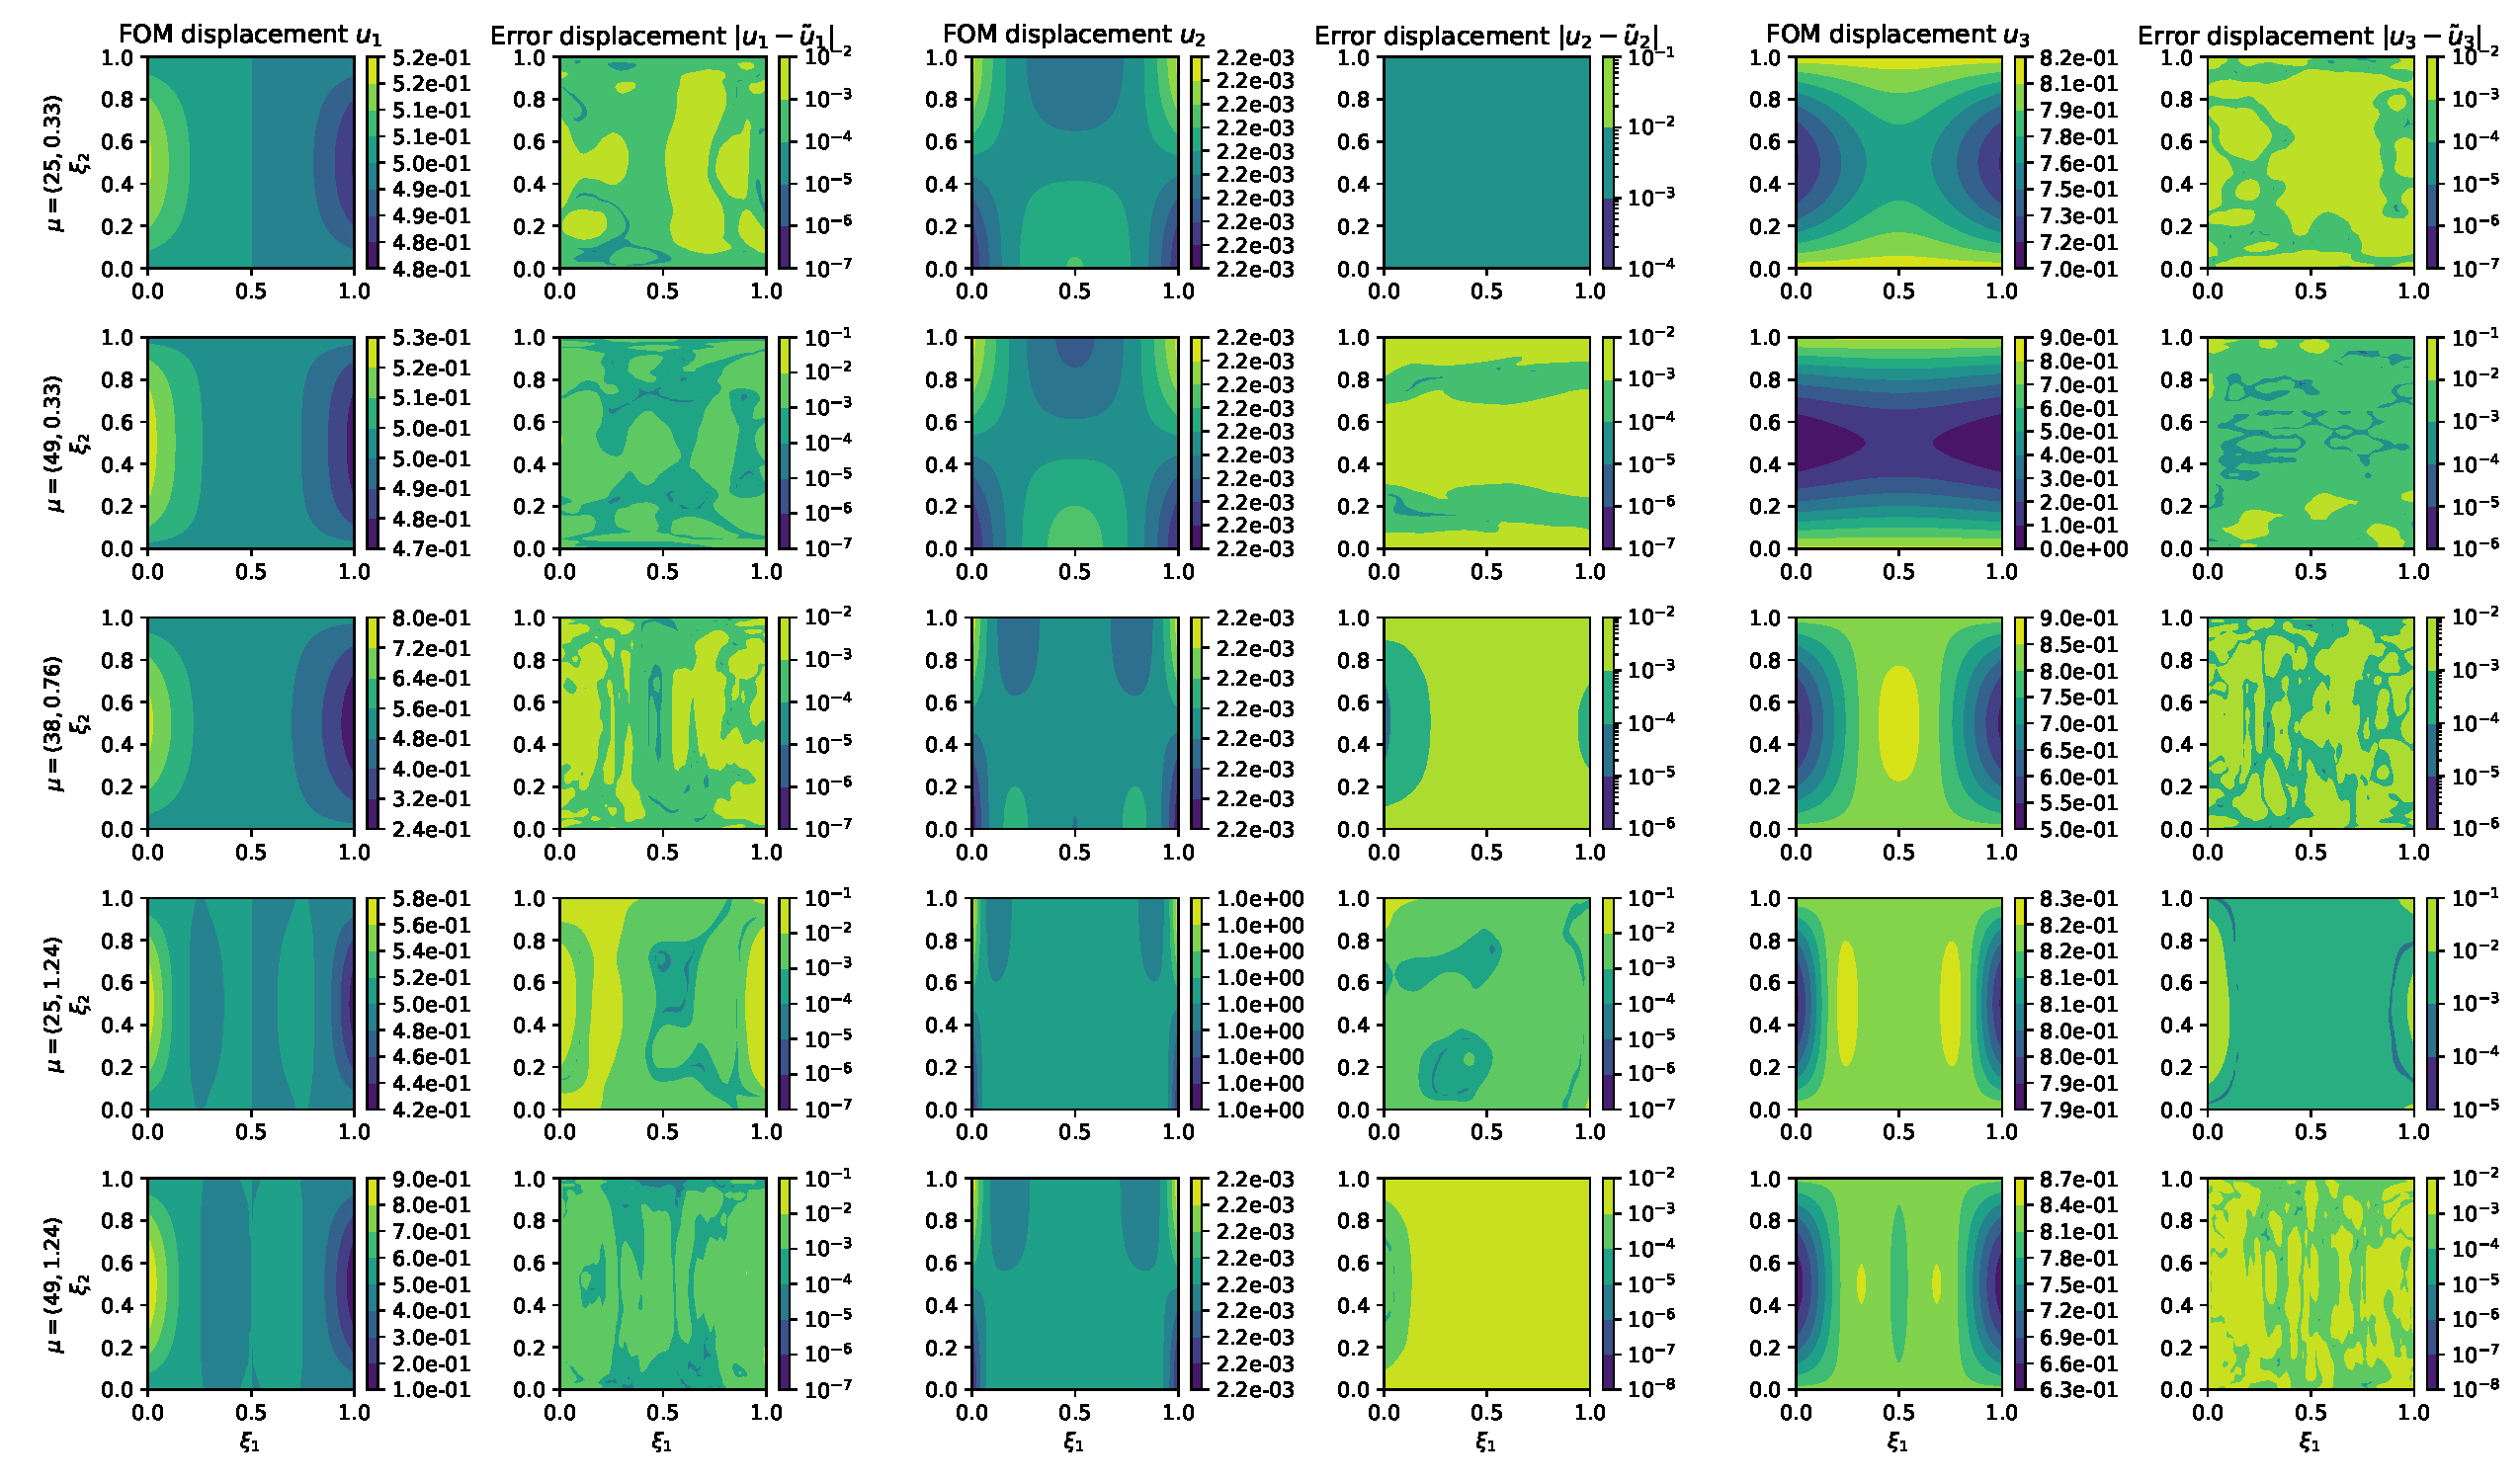
\includegraphics[width=1.3\textwidth]{imgs/kirchoff_pinn_trained.pdf}}
    \caption{Example of trained UC-USM-Net. On different rows there are different choices of $\boldsymbol \mu$. On different columns there are represented the three components of the displacement with respective error. Hyperparameters: depth=10, width=100, activation=ELU, $N_t=$3.2e5, batch size=128, epochs=200.}
    \label{fig:usmnet-kirchoff-trained}
\end{figure}

The unrolled dataset contains 8~192~000 samples. I start by using a UC-USM-Net with input the parametric coordinates $\boldsymbol \xi$. If not stated otherwise the training is stopped after 200 epochs. Exploiting the results obtained in Section \ref{sec:usmnet-lapl} I test as activation just the ELU and the Tanh functions, I also test different depth and width of the model.


\begin{center}
\begin{tabular}{ |c|c|c|c|c|c|c| } 
 &&&\multicolumn{2}{c|}{ELU} &\multicolumn{2}{c|}{Tanh}\\
 $N_t$ & size & avg train time [s] & $l^1$ & $l^2$ & $l^1$ & $l^2$\\ 
 \hline
 8e4&$8 \times 80$  &719& 1.09e-3 & 9.03e-3 & 1.07e-3 & 8.04e-3 \\
 8e4&$9 \times 90$  &842& 1.20e-3 & 6.35e-3 & 1.11e-3 & 8.85e-3 \\
 8e4&$10 \times 100$ &933& 8.54e-4 & 5.51e-3 & 1.58e-3 & 1.31e-2 \\
\end{tabular}
\end{center}

Then I test different batch sizes for different sizes of the training dataset.
\begin{center}
\begin{tabular}{ |c|c|c|c|c|c|c|c|c| } 
 &&&\multicolumn{2}{c|}{Batch: 8} &\multicolumn{2}{c|}{Batch: 16} &\multicolumn{2}{c|}{Batch: 32}\\
 $N_t$ & size & activation & $l^1$ & $l^2$ & $l^1$ & $l^2$ & $l^1$ & $l^2$ \\ 
 \hline
 1e4&$7 \times 70$ & ELU & 1.86e-3 & 1.46e-2 & 1.75e-3 & 1.41e-2 & 1.68e-3 & 1.35e-2\\
 2e4&$7 \times 70$ & ELU & 1.30e-3 & 1.31e-2 & 1.28e-3 & 1.30e-2 & 1.58e-3 & 1.14e-2\\
 4e4&$7 \times 70$ & ELU & 1.06e-3 & 1.89e-2 & 1.13e-3 & 8.27e-2 & 9.72e-4 & 6.64e-3\\
 8e4&$7 \times 70$ & ELU & 7.40e-4 & 5.52e-3 & 9.15e-4 & 6.71e-3 & 9.23e-4 & 6.63e-3\\
\end{tabular}
\end{center}

Since increasing the training dataset size improves the training but is also very expensive, I test the trade-off of increasing $N_t$ while increasing also the batch size.

\begin{center}
\begin{tabular}{ c|c|c|c|c|c|c } 
 $N_t$ & batch size & size & activation & train time [s] & $l^1$ & $l^2$ \\ 
  \hline
 8e4 & 32 & $10 \times 100$ & ELU & 968.08 & 8.54e-4& 5.51e-3 \\
 8e4 & 64 & $10 \times 100$ & ELU & 580.37 & 1.15e-3&  9.85e-3 \\
 16e4 & 32 & $10 \times 100$ & ELU & 1951.5 & 7.59e-4&  5.80e-3 \\
 32e4 & 128 & $10 \times 100$ & ELU & 1636.2 & 5.02e-4&  1.57e-3 \\
 
\end{tabular}
\end{center}
The last model reported in this table is shown in Figure \ref{fig:usmnet-kirchoff-trained}. Training it for 400 epochs I obtain a model with the following error metrics: $l^1=3.79$e-4 and $l^2=9.85$e-4. Finally, I test the results on a PC-USM-Net and compare it to the UC-USM-Net. I stress that in PC-USM-Net there is one extra input since $\boldsymbol \xi \in \mathbb R^2$ and $\mathbf x \in \mathbb R^3$.

\begin{center}
\begin{tabular}{ |c|c|c|c|c|c| } 
 &&\multicolumn{2}{c|}{UC-USM} &\multicolumn{2}{c|}{PC-USM}\\
 $N_t$ & size & $l^1$ & $l^2$ & $l^1$ & $l^2$\\ 
 \hline
 8e4&$9 \times 90$  & 1.20e-3 & 6.35e-3 & 1.53e-3 & 1.23e-2 \\
 8e4&$10 \times 100$ & 8.54e-4 & 5.51e-3 & 1.05e-3 & 1.15e-2 \\
\end{tabular}
\end{center}


The UC-USM-Net in this case achieves a much smaller error metric, corroborating the hypothesis of \cite{regazzoni2022} that using the parametric coordinates improves the model accuracy.





\section{Discussion}\label{sec:discussion}
I have compared DL-ROM and USM-Net as methods for creating ROM of parameterized PDEs. Specifically, I have tested their performance on two model problems with a domain parameterized by a NURBS surface: a Poisson's equation and the Scordelis-Lo roof benchmark (a vectorial problem on a 2D surface immersed in a 3D space).

I have found that USM-Net perform better both in terms of accuracy and computational cost with respect the simplified version of DL-ROM I have implemented. The gain is more evident in the second test case, where the USM-Net are able to leverage the 2D parameterization of the 3D geometry. Moreover, USM-Nets are more flexible, being able to exploit physic-informed regularization and physical measurements. My results agree with \cite{regazzoni2022} and show that UC-USM-Net perform better than PC-USM-Net. Finally, I have shown that the physical mapping $\Psi_{\mathcal G}$ can be learned through a neural network, in order to exploit physic-informed regularization.

Possible improvements include: confronting the original DL-ROM with USM-Net, pre-training, raising training dataset size for USM-Net, applying hard constraints \cite{lu2021physics} for USM-Net; implement physical regularized (PINN-like \cite{raissi2019physics}) for USM-Net. 

Code is available at \href{https://github.com/MatteoCaldana/mm4dl-project}{mm4dl-project}.


%%
%\clearpage
\bibliographystyle{plain}
\bibliography{bibl}

\end{document}